%!TEX root = thesis.tex

%:-------------------------- Preamble -----------------------

% Three languages are supported, which will be reflected in the logo on the front page. Pass the appropriate language
% specified as a class option to uit-thesis. Passing any other languages supported by babel will result in the default
% language on the frontpage. If no language is passed, the default is selected.
%  - USenglish (default)
%  - norsk
%  - samin
% The frontpage comes in two variants, Master's thesis and PhD. Master is default, use classoption 'phd' for the PhD version.
\documentclass[USenglish]{uit-thesis}
\renewcommand{\bibname}{References}
% Lorem ipsum
\usepackage{lipsum}
\usepackage{appendix}
\usepackage{amsthm}
\usepackage{hyperref}
\usepackage{tikz}
\usepackage{pgf-umlsd}
\usepackage{float}
\usepackage{listings}
\usepackage{caption}
\usepackage{subcaption}
\usepackage{amsmath}
\usepgflibrary{arrows}
\usepackage{listings}
\usepackage{amssymb}
\usepackage{enumitem}  

\usepackage{glossaries}

\newtheorem{defs}{Definition}

\makeglossaries

% Add external glossaryentries

\loadglsentries{acronyms}

\newglossaryentry{thesis}
{
  name=thesis,
  description={
    },
}
\newglossaryentry{lage}
{
  name={long ass glossary entry},
  description={
  },
}


\newcommand{\listdefinitionname}{My list of definitions}
\newlistof{definition}{def}{\listdefinitionname}
\newcommand{\definition}[1]{%
  \refstepcounter{definition}%
  \par\noindent\textbf{The Definition~\thedefinition. #1}%
  \addcontentsline{def}{definition}
    {\protect\numberline{\thechapter.\thedefinition}#1}\par%
}

\def\bitcoin{\leavevmode\rlap{\hskip.5pt-}B}

\def\bitcoinA{%
	\leavevmode
	\vtop{\offinterlineskip %\bfseries
		\setbox0=\hbox{B}%
		\setbox2=\hbox to\wd0{\hfil\hskip-.03em
			\vrule height .3ex width .15ex\hskip .08em
			\vrule height .3ex width .15ex\hfil}
		\vbox{\copy2\box0}\box2}}

\def\bitcoinB{\leavevmode
	{\setbox0=\hbox{\textsf{B}}%
		\dimen0\ht0 \advance\dimen0 0.2ex
		\ooalign{\hfil \box0\hfil\cr
			\hfil\vrule height \dimen0 depth.2ex\hfil\cr
		}%
	}%
}



\begin{document}
\renewcommand{\bibname}{References}
%:-------------------------- Frontpage ------------------------

% \title{Understanding Digital Currencies and Blockchain}
\title{Trading Network Performance for Cash in the Bitcoin Blockchain}
\subtitle{subtitle}			% Optional
\author{Enrico Tedeschi}
\thesisfaculty{Faculty of Science and Technology \\ Department of Computer Science}
\thesisprogramme{Master Thesis in Computer Science}
%\ThesisFrontpageImage{img/}	% Optional

\maketitle

%:-------------------------- Frontmatter -----------------------
\frontmatter

%\begin{dedication}
%Dedication here
%\end{dedication}

%\begin{epigraph}
%\epigraphitem{Simplicity is prerequisite for reliability.}{Edsger Dijkstra}
%\epigraphitem{Beware of bugs in the above code;\\I have only proved it correct, not tried it.}{Donald Knuth}
%\end{epigraph}

%TODO: SUBSTITUTE ALL THE # WITH CORRECT NUMBERS
\begin{abstract}
\label{sec:abstract}
%TODO: change abstract accordingly to the results

%TODO: Short introduction to blockchain
Nowadays blockchain systems are emerging and they are spreading
each day more. Cryptocurrencies are the biggest example
of a physical implementation of this protocol, having in $2012$ more
than $50$ thousands transactions per day and reaching now
in $2017$ more than $350$ thousands of transactions approved every day.
In this thesis we
evaluate the most famous blockchain system, the \emph{Bitcoin blockchain}.
Public blockchains have emerged as a plausible messaging substrate
for applications that require highly reliable communication.
However, sending messages over existing blockchains can be cumbersome
and costly as miners require payment to establish consensus on the
sequence of messages. The blockchain protocol requires an always
growing size of the informations stored in it so its \emph{scalability} is
the biggest problem. For that reason we collected data to be analyzed and
stored in our own dataframe, saving up to $x10$ space
for the analysis.

%TODO: Previous works, problems on blockchain and what we did so far
This thesis will consider the network
performance of the Bitcoin public ledger when used as a massaging
substrate. From $2009$ to $2017$ a lot of analysis has been done on
Bitcoin blockchain and meanwhile its block size limit changed multiple times,
from $256$\,bytes up to $1$\,Mb,
the Bitcoin price raised from $\sim$\,$0.7$\,\$ to more than $4.000$\,\$ and
different papers were published discussing whether changing or not the block size
limit or talking about the fees a miner could get from clients.
We read and considered previous analysis on Bitcoin blockchain,
we then present our own dataset, which contains a significant portion of
the Bitcoin blockchain, updated at $09$-$2017$,
discuss our results and compare them with other evaluations
from past years,
then we also discuss how the fee paid to miners evolves
during time and how much a
client could pay for a faster approval time, plus we take into consideration
transaction visibility, blockchain growth and fees paid to miners.
From this we propose
and evaluate, using machine learning techniques,
three different cost prediction models for predicting
bandwidth per Bitcoin cost of upcoming transaction. The models can
be used by application to throttle network traffic to optimize
message delivery. We also discuss and consider, according to the data
obtained, whether the block size limit should be increased for an higher
\emph{throughput} or not.

%TODO: 
People are using Bitcoin because 
it has a lower fee rate and no central authority, we aim to find any
possible relation between the fee paid from a transaction to a
miner and the approval time of this transaction, plus we also noticed that
the bigger is the blockchain size the more the system become
centralized, since only few members, or nodes, of the Peer to Peer network can
support and use the full blockchain.

Bitcoin blockchain has been analyzed with a blockchain analytics system,
developed using Bitcoin's API and data were collected both by using the
API and parsing \url{blockchain.info} HTML pages.
A total of \# transactions has been evaluated, more transactions than ever were
considered before and useful informations about the Bitcoin blockchain emerged.
This thesis gives also a measurement about accuracy of data
provided from \url{blockchain.info}.
\end{abstract}

%\begin{acknowledgement}
%
%\end{acknowledgement}

\tableofcontents

\listofdefinition

%:-------------------------- Mainmatter -----------------------
\mainmatter
\chapter{Introduction}
\label{chap:introduction}
%TODO: INSERT: Bitcoin has the unintuitive property that while the ownership of money is implicitly anonymous, its flow is globally visible\,\cite{Meiklejohn:2013}.

%TODO: give a short example of previous work, what they did and show that this problem has relevance for this field! works might be: Rizun one, Bohme (longitudinal study of bitcoin transaction fees) and On scaling decentralized blockchain system.

%TODO: Another question we asked ourself for the data is how the various attributes relate to one another, and a quick way to get an idea of pair-wise relationship is to cross-plot the attributes and later interpolate the results.

%TODO: ADJUST INTRODUCTION
In $1964$, Paul Baran\,\cite{Baran1964:ODC}
represented a very clear topology describing the differences
between a centralized, decentralized and distributed
network~(Figure\,\ref{fig:networks}). Since then, the attention
in developing systems moved from a centralized scheme to a distributed one,
leaving most of the computation to every single user in the network
rather than a central coordinator.
Such a change might be easy for systems that do not require much of
security, where authentication or authorization is minimal.
However, the more a system needs to be secure, the more the decentralization
process might be tricky as it becomes very important to rely on
some trusted central coordinator. Systems that more than others need
to be secure are the one related to e-commerce, banking and trades, all
systems that have to deal with money.

\begin{figure}[h!]
	\centering
	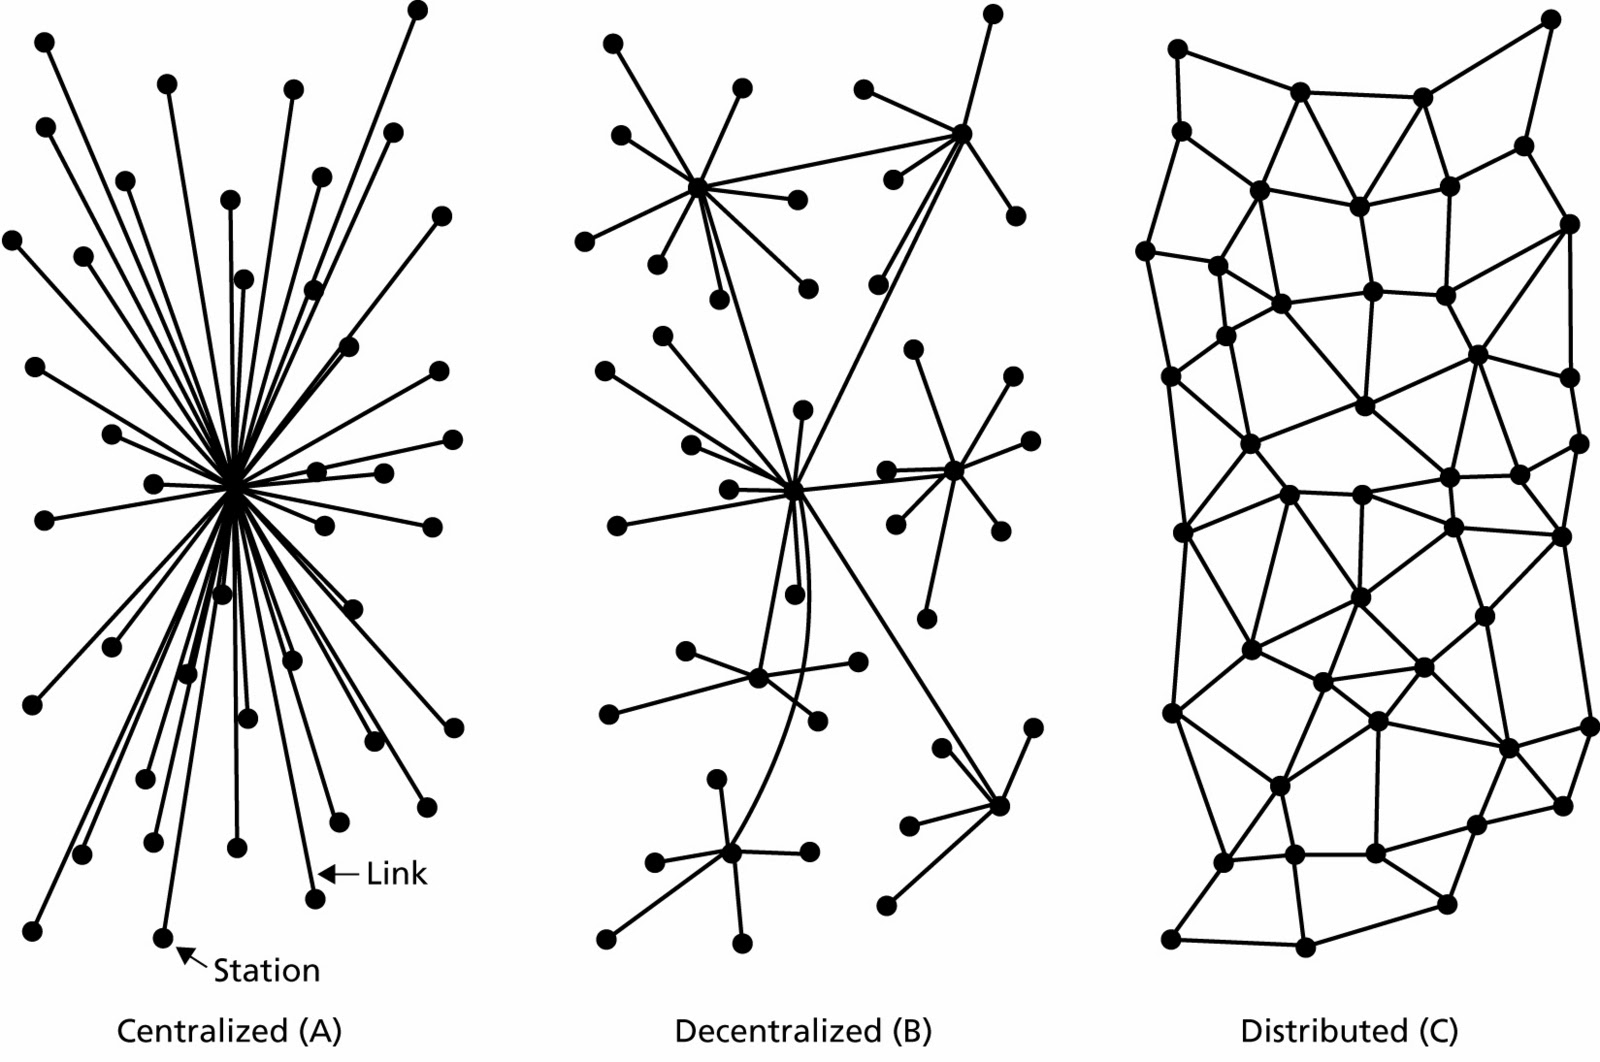
\includegraphics[width=1\textwidth]{img/networks}
	\caption{Differences between network topologies. Source: On Distributed
		Communication Networks, Paul Baran, 1964.}
	\label{fig:networks}
\end{figure}

In $1983$, a research paper by David Chaum introduced the idea of digital cash\,\cite{chaum83blindsign}. In $1990$ he founded \emph{DigiCash},
an electronic cash company that closed because of bankrupt in
$1998$. After that, other systems such as \emph{e-gold} ($1996$) and
\emph{PayPal} ($1998$) emerged. However, these systems allowed
digital money transfer while they were still relying on a central authority.
In $2008$ Satoshi~Nakatomo has presented Bitcoin\,\cite{Nakamoto_bitcoin},
the first decentralized digital currency.
Until $2008$ e-commerce used to rely exclusively on financial institutions
serving as trusted third parties. Those are involved in the electronic
payments process and they have to guarantee consistency of the
transactions and security of data.

Decentralized digital currencies are not
dependent on any trusted third parties and they are built over a
\gls{p2p} network where every component has the same
privileges. These systems allow money exchange
without a central authority, which means lower fees, no geographical
separation and global trust among users. After Bitcoin,
more decentralized digital currencies emerged, in $2011$ \emph{Litecoin},
originally based on the bitcoin protocol, then in $2013$
Gavin~Wood has presented \emph{Ethereum}\,\cite{ethereum} and in
$2014$ \emph{Monero} currency was released.

The order of transaction is essential in any cryptocurrency systems. 
However, establishing correct order can be problematic in
decentralized cryptocurrency systems as they allow 
arbitrary nodes to join, including nodes that might be malicious.
If arbitrary or Byzantine faults are allowed, the system might be left in an inconsistent or invalid state\,\cite{Lamport1982}.
The ability to mask Byzantine faults has been implemented in various systems such as
Byzantium\,\cite{Garcia:2011:EMB}, HRDB\,\cite{vandiver2007hrdb} and MITRA\,\cite{Luiz:2014:MBF}.
These protocol guarantees consistency of transactions having
$f$ faulty nodes, with a total of $N$ nodes where $N=2f+1$ or $N=3f+1$, and
a protocol like \emph{Fireflies}\,\cite{Johansen2015Fireflies} provides secure and
scalable membership management and communication substrate in overlay
network with Byzantine members. To guarantee an order of
transaction all these cryptocurrencies rely on the \emph{blockchain} protocol.

\section{Blockchains}
\label{sec:blockchains}
The need to tolerate malicious members was the reason for introducing
the \emph{blockchain} into cryptocurrency systems. The fundamental principle 
behind the blockchain is that consensus on transaction ordering is based on 
contributed computational power rather than number of participants. 
The blockchain works by appending
transactions in blocks. Every block is generated after a relevant computation
(\emph{proof-of-work}),
and each new block is appended to the public ledger of data,
the blockchain, having in that way an ever growing chain of data
containing every transaction ever happened.

Besides its use in cryptocurrency, this blockchain technology
opens up to several usages in different sectors such as
trading, file storage or identity management. Indeed it is already
used by NASDAQ in its private socket market.  If used in a \gls{p2p}
file sharing network, the blockchain removes the need of a centralized
data base and heavy storage areas. Moreover it allows users to create
tamper-proof digital identities for themselves.
Blockchain technology opens up to usages in several important sectors
such as trading, file storage, and identity management.

Blockchains essentially implements a distributed consensus protocols that enable a set of untrusted processes to agree on the content of an append only data structures. 
These ledgers are divided into blocks and linked together in sequence by hashes. 
They facilitate transactions between consenting individuals who would otherwise have no means to trust each other and deal with geographical separation and interfacing difficulties 
This technology promises a highly resilient and communication substrate where messages are kept potentially for a long time.

Nonetheless, decentralized digital currencies also have some side effects.
The most relevant is \emph{scalability}, due to the steady growth of the
blockchain. It should be also considered that
decentralized cryptocurrencies operate in open (or permissionless) networks
in which the ledger of data could be manipulated from arbitrary adversaries and
according also to the paper from University of Singapore\,\cite{Luu:2016}
security of smart contracts has not received much attention yet. And since the
only part not protected from cryptography is the \emph{order of transactions}\,\cite{ethereum_white_paper},
an attacker would try to convince the network that a transaction
occurred earlier than another one to gain money.
The security bugs in smart contracts are classified as \emph{Transaction-Ordering Dependence},
\emph{Timestamp Dependence}, \emph{Mishandled Exceptions}
and \emph{Reentrancy Vulnerability}\,\cite{Luu:2016}.
In this thesis we refrain from explaining Bitcoin and its terminology in detail
and refer the reader to already existing high-level\,\cite{Underwood:2016:BBB,
Bohme2015BETG}
or technical\,\cite{Nakamoto_bitcoin, ethereum_white_paper}.
 description.
\section{Problem Statement}
\label{sec:probdefinition}
%TODO: One of the most recent debate on Bitcoin blockchain is wether the block size $Q$ should be increased or not. Rizun\,\cite{Rizun:2015:blocksizelimit} in his paper explained how challenging might be the increment of the block size and it defines an optimal size of~$\sim$\,$1$\,Mb. Anyway there are arguments in favor of increasing the block size, we analyzed these arguments and discuss whether and where is conveninet to increase the $Q$. Pros: More transactions per second, higher throughput. Less fees. Cons: miner won't get enough fee. Higher (exponential) risk of orphaning.

While doing research, studying and reading papers related to blockchains,
it turned out that the most urgent concerns are related to
its scalability and performance, but also to the fee
a client has to pay to get better latency.
In $2015$, Möser and Böhme write\,\cite{Moser2015}:
\begin{quote}
	\emph{Bitcoin may not be as cheap for consumers as it appears.}
	[\dots]
	\emph{Bitcoin users are encouraged to pay fees to miners, up
	to $10$\,cents (\gls{usd}), per trnsaction, irrispective of the amount
paid.}
\end{quote}

Rizun writes in $2015$\,\cite{Rizun:2015:blocksizelimit}:
\begin{quote}
	\emph{The block size limit was set at one megabyte, corresponding
		roughly to three transactions per second.}
		[\dots]
		\emph{The transaction rate is over three hundred times larger
		than when the block size limit was introduced, and rising the limit
		is now being seriously considered.}
\end{quote}
Then Croman writes in $2016$\,\cite{croman2016}:
\begin{quote}
\emph{The current trend of increasing the block sizes on Bitcoin protends
a potential problem where the system will reach its maximum capacity to clear
transactions, probably by $2017$.}
\end{quote}

%TODO: REVIEW THIS:
It is obvious then that these problems need to be taken
into consideration.
In this thesis we discuss the scalability of the blockchain, how it affects
the throughput and we present performance observations of the
Bitcoin blockchain, analyzed with a blcockhain analytic system developed
for this purpose. We provide detailed insights and analysis on how
Bitcoin's characteristics, such as fee, block size and reward to different
miners involved have changed over time, and provide an
updated model describing how the Bitcoin blockchain will grow. 
We analyzed the correlation between the fee paid from a transaction
and its \emph{latency}, or the time it takes to 
be visible in the whole network.
%TODO: THREE MODELS? KEEP THEM?
Three different models are proposed to describe how applications
best can spend money to improve network charactertics,
this affects average bandwidth available to an application. 

%TODO: keep it or not?
\subsection{Scalability}
\label{sec:prob_stat_scalability}
Scalability and network performances are urgent
concern in existing Blockchain-based
cryptocurrencies~\cite{croman2016}.
According to Ethereum white paper\,\cite{ethereum_white_paper},
if Bitcoin would have the same amount of transactions
of a VISA circuit, its blockchain would grow
about $1$\,Mb every $3$ seconds, $\sim$\,$28$GB per day,
instead of the actual growth of $\sim$\,$0.12$GB per day.
In this thesis we discuss how much scalability affects
centralization in Bitcoin network and how much it will
impact in the next couple of years the blockchain
growth.
%TODO: Transactions-wise experiments or blocks-wise experiment

\subsection{Performance}
Centralized schemes, like VISA are immediate, while having a
throughput of $2000$\,transactions/sec
up to $56$ thousands\,transactions/sec\,\cite{croman2016}.
It is true that Bitcoin has lower fees than centralized
currency schemes, but these properties
come at a performance and scalability cost.
In the paper from Croman\,\cite{croman2016}, they
claim that Bitcoin achieve a throughput of $7$ transactions/sec.
In this thesis we also want to update at $2017$ this statment
and see how much a block size change might
influence the whole network performance.

%TODO: Sentences:
% You can't build something that works without having a certain level of centralization, there always should
% be a compromise between centralization and how much you can trust spontaneous orders to take over.

%\begin{quote}
%\emph
%{applications can control available bandwidth by paying mining fees.}
%\end{quote}


\section{Method / Context}
\label{sec:method}
%TODO: REVIEW THIS
In this thesis we analyze a considerable part of the blockchain.
In the paper from $2015$ written by Möser and Böhme\,\cite{Moser2015},
they analyze tips and tolls in Bitcoin blockchain, they collected data until $2014$
and they analyze more than $9$\,million of transactions.
At that time there were a total of $100$\,thousands
transactions per day, while today we count about $350$\,thousands
txs/day, so the retrieving part turned out to be more time consuming than expected.
Despite that, we aim to collect even
a larger portion of the blockchain, storing data smartly in a
\emph{data frame}, which allows us to spare
up to $10x$ of the space the blockchain actually requires. Then we analyze data
and with \emph{machine learning} techniques we define models, discuss about
the results and how much they can be reliable in a future-wise implementation.
In our data frame we store more than \# transactions, with an analysis in between
\#date and \#date.
We used for the information retrieval \gls{api} from \url{blockchain.info}
combined with a \gls{html} parsing on every "block-page"
of the same website.

Our assumption is that we can get sufficient information about the
blockchain growth, the block creation time, the time for a transaction to be visible
in the public ledger of data and which miners are the more trendy and
which usually requires more fee by retrieving and analyzing only a portion
of the blockchain, but having in that way a finer
granularity than the one represented in the Bitcoin website. In that
way we hope to gain more informations out of it.
Moreover, sampling data from a single node in the blockchain gives statistics
representative of the whole system.

For the analysis, data are retrieved block per block and part of the blockchain
is saved in a text file. This finer granularity allows us to have
a lot of informations that may be hidden in the statistical analysis
provided from Bitcoin. It is also possible to use the informations retrieved
to make future predictions about how much the 
Bitcoin blockchain will grow, using polynomial interpolation on the data. According
on how many blocks ago are fetched, it is possible to have an accurate prediction
on the blockchain growth for the next few years.

We are going to compare more recent data, retrieved real time, with the Bitcoin one and see the differences of the
blockchain growth. Moreover, In the Bitcoin website for blockchain analysis,
\url{blockchain.info}~\cite{bitcoin_blockchain}, the finer granularity
shows data for the last $7$ days while we are collecting and monitoring data
at every block creation ($\sim8$-$10$ min). In that way is easier for us to check
if there are any abnormalities in the ledger of public data.

\section{Outline}
\label{sec:outline}
%This chapter introduces the Blockchain, blocks, mining, fee and other key words related to
%decentralized digital currencies. Chaper~\ref{chap:techback} gives a detailed explanation
%on the main aspects of this new technology and how decentralized
%cryptocurrencies work. It will talk about consensus protocol, data structure, mining
%process, gas, fees and proof of work. Chapter~\ref{chap:expsetup} explains how the blockchain
%analytics system was designed and implemented, which data are
%taken into consideration and why and also how data are retrieved and
%organized into text files. Chapter~\ref{chap:evaluation} talks about the
%evaluation and the results of the data analysis. It shows the plots generated with some
%consideration and the comparison between the expected results from the Bitcoin blockchain.
%Plus, prediction models obtained with statistical analysis are showed.
%Finally, Chapter~\ref{chap:conclusion} includes future implementation of the system,
%possible development of this project and conclusions of the overall work.

%TODO: PREVIOUS WORK -- WORKING ON THIS CHAPTER
\chapter{Related Works - SotA}
\label{chap:prev_works}
%TODO: Talks about more papers on bitcoin
As mentioned in Chapter\,\ref{chap:introduction},
scalability and analysis on the blockchain has been taken into consideration
by many researchers in the past years.
This chapter summarizes the most relevant papers or
works that talks about Bitcoin,
blockchain and decentralized cryptocurrencies,
it gives a short view of what has already been done and
the reults obtained.
In our previous paper\,\cite{Tedeschi:2016:PBB}, we enhance
the importance of paying for having a certain
bandwidth in the Bitcoin network.
A paper
from Peter~R.~Rizun\,\cite{Rizun:2015:blocksizelimit},
explains how a rational Bitcoin
miner should select transactions from his node mempool,
when creating a new block,
in order to maximize his profit. We discuss that and apply
new data from more recent sources to this idea of
"selecting the right transaction" in a way that a miner could
select the right transactions to earn more money out of the whole
mining process.
Scalability has taken into consideration
in the Position Paper of Kyle Croman\,\cite{croman2016}, they
analyze how fundamental bottlenecks in Bitcoin limit the ability
of its current peer-to-peer
overlay network to support substantially higher
throughputs and lower latencies. We are
going to test the throughput as well, comparing it with the one
showed in this paper.
Regarding fees and tolls paid in the Bitcoin blockchain
we refer to the study done in $2014$ from Möser and
Böhme\,\cite{Moser2015}. They analyze the
entire blockchain and make assumptions about
that these "fees" are supposed to substitute miners'
minting rewards in the long run. This paper
contributes empirical evidence from a historical
analysis of agents' revealed behavior concerning
their payment of transaction fees.
Furthermore, to fully understand how is possible
to make money out of the blockchain and mining,
in necessary to have a view of
how \emph{VISA}\,\cite{visa} makes money as well.

\section{Rizun - A Transaction Fee Market Exists Without a Block Size Limit}
\label{sec:rizun}
\subsection{Problems}
A pressing concern exists over the ramifications of changing (or not)
a Bitcoin protocol rule called \emph{block size limit}. This rule sets an
upper bound on the network's transactional capacity, or \emph{throughput}.
The limit was set at $1$\,Mb, corresponding roughly to three transactions
per second. When this limit was set, it was over eight hundred times
greater than what was required. However in $2015$, blocks
were filled near capacity and users experienced delays. In $2015$
the transaction rate was over three hundred times larger
than when the block size limit was introduced. One of the
concerns is whether, in the absence of a limit or if the limit
is far above the transactional demand, a healthy transaction
fee market would develop which charges users the full
cost to post transactions. The object
of this paper is to consider whether or not such a fee
market is likely to emerge if miners, rather than the protocol,
limit the block size.
\subsection{Methods}
This paper shows how a Bitcoin miner should
select transactions from his node's mempool
when creating a new block in order to maximize
his profit in the absence of a block size limit.
\emph{Block space supply curve} and
\emph{mempool demand curve} are explained, and the
paper shows how the supply and demand
curves from classical economics are related to the
derivatives of these two curves.
In the paper Rizun claims that the block-size limit determines the
transaction throughput. In this paper he derives
the \emph{miner's profit equation} and then
he introduces two novel concepts called
the \emph{mempool demand curve} and the
\emph{block space supply curve}.
\subsubsection{Miner's Profit Equation}
Every time a block is mined, the miner expects to generate a revenue $\langle V \rangle$
at hashing cost $\langle C \rangle$ to earn profit per block
\begin{equation}
\label{eq:minerprofit}
\langle \Pi \rangle = \langle V\rangle - \langle C\rangle.
\end{equation}
Miner's profit equation in~\ref{eq:minerprofit} shows the gain of a miner $\langle \Pi \rangle$,
where the hashing cost is represented as follows:
\begin{equation}
\label{eq:hashingcost}
\langle C\rangle = \eta hT.
\end{equation}
So the hashing cost $\langle C\rangle$ is directly dependent from the miner's individual hash rate, $h$,
the cost per hash, $\eta$, and the creation time, $T$. Moreover, is important to consider the
expectation value of a miner's revenue per block, this value is represented with $\langle V\rangle$
and is equal to the amount he would earn if he won the block multiplied by his probability of
winning. So the expected revenue would be:
$\langle V\rangle = (R + M) h/H$,
where the amount he would earn is the sum of the block reward, $R$, and the transaction fees, $M$.
His probability of winning, assuming all blocks propagating instantly, is equal to the ratio of his hash
rate, $h$, to the total hash rate of the Bitcoin network, $H$. The problem with this equation is that it
does not reflect the miner's diminished chances of winning if he chooses to publish a block that propagates
slowly to the other miners. If a miner finds first a valid block, but his solution is received after most miners
are working on another, then his block will likely be discarded. This effect is called \emph{orphaning}. The
equation, considering the orphaning factor, $\mathbb{P}_{orphan}$, is the following:
\begin{equation}
\label{eq:expectedrevenue}
\langle V\rangle = \left(R + M\right)\frac{h}{H}\left(1 - \mathbb{P}_{orphan}\right).
\end{equation}
Where $P_{orphan}$ increases with the amount of time a block takes
to propagate to other miners. Indeed, if $\tau$ is
the block propagation time, the
probability of orphaning is defined as:
\begin{equation}
\label{eq:orphaning}
\mathbb{P}_{orphan} = 1 - e^{-\frac{\tau}{T}}.
\end{equation}
In conclusion the \emph{miner's profit equation} is defined as:
\begin{equation}
\label{eq:minerprofiteq}
\langle \Pi \rangle = (R + M)\frac{h}{H} e^{-\frac{\tau}{T}} -\eta hT
\end{equation}
A \emph{rational miner} selects which transactions to include in his block in a manner that maximizes
the expectation value of his profit. This selection is explained with the \emph{mempool demand curve}
and the \emph{block space supply curve}.

\subsubsection{The Mempool Demand Curve}
\label{sec:mempooldemand}
The set of transactions that still need to be approved and included
in a block is called \emph{mempool}.
The mempool set is denoted with $\mathcal{N}$ and the number
of transactions contained within it as $n$.
According to the size limit, a block can select a $b \leq n$
transactions from $\mathcal{N}$ to create a
new block $\mathcal{B} \subset \mathcal{N}$.
A block first includes transactions with an higher \emph{fee density}, $\rho$.
This last, is a ratio between
the \emph{transaction fee}, $t_f$ and the \emph{transaction size}, $t_q$.
To construct the mempool demand
curve, is necessary first sorting the mempool from
greatest fee density to least and then
associating an index $\{i: 1,2,\dots,n-1,n\}$ with each
transaction in the resulting list.
The mempool demand curve will be then a graphical
representation of the sum of the fees offered
by each transaction in this sorted list:
\begin{equation}
\label{eq:memdemandcurve}
M_{demand}(b) \equiv \sum_{i=1}^{b} fee_i,
\end{equation}
and the sum of each transaction's size in bytes:
\begin{equation}
\label{eq:transactionsize}
Q(b) \equiv \sum_{i = 1}^{b} size_i.
\end{equation}
The mempool demand curve represents then the maximum fee,
$M_{demand}(b)$
a miner can claim by producing a given quantity $Q(b)$ of blockspace.
%TODO: Insert graph of the mempool demand curve

\subsubsection{The Block Space Supply Curve}
\label{sec:blockspacesupply}
The size of the block a miner elects to produce controls the fees he attempts to claim, $M(Q)$,
and the propagation time he chooses to risk, $\tau(Q)$. The block space supply curve represents
the fees a miner requires to cover the additional cost of supplying block space $Q$. This cost grows
exponentially with the propagation time. The equation which represents this curve is the
following:
\begin{equation}
\label{eq:blockspacesupply}
M_{supply}(Q) = R\left(e^{\frac{\Delta \tau (Q)}{T}} - 1\right),
\end{equation}
where $\Delta \tau (Q) \equiv \tau(Q) - \tau(0)$. The propagation time ,$\tau$, is just an esteem from
the propagation delay versus the block size.

\subsubsection{Maximizing the Miner's Profit}
To maximize his profit, the miner construct a mempool
demand curve and a space supply curve.
The block size $Q^*$ where the miner's surplus,
$M_{demand} - M_{supply}$, is largest represents
the point of maximum profit. Considering this point $Q^*$ of maximum
profit, Rizun considers three market conditions for Bitcoin transaction
fees: \emph{healthy}, \emph{unhealthy} and \emph{non-existent}.
In a healthy fee market, the miner's surplus is maximized
at a finite quantity of block space, and thus a miner is
incentivized to produce a finite block. In an unhealthy
market, the miner's surplus continually increases with
block space, and therefore a rational miner should produce
an arbitrary large block. In a non-existent market,
including \emph{any} transactions results in a deficit
to the miner, and so the miner is better off
producing an empty block. A rational
miner will produce a big block if his mempool
is full of high fee density transactions, and
will produce an empty block if no transactions pay a fee sufficient
to offset the orphaning risk.

\subsection{Results}
%TODO: Conclusions from this paper
In conclusion, they show that a transaction fee market should
emerge without a block size limit if miners
include transactions in a manner that maximizes
the expectation value of their profit. A
critical step in establishing this result was their
calculation of the miner’s cost to supply
additional block space by accounting for orphaning risk.

\section{Möser \& Böhme - Trends, Tips, Tolls: A Longitudinal
study of Bitcoin Transaction Fees}
\label{sec:moser}
\subsection{Problems}
The Bitcoin protocol supports optional direct payments
from transaction partners to miners, also called \emph{fees}.
Acknowledging their
role for the stability of the system, the right level of
transaction fees is a hot topic of normative debate. The actual
costs of the system are not extensively studied yet. Disregarding
intangible factors of (in)convenience, Bitcoin may not be as cheap for
consumers as it appears. The main problems/questions
that this paper focuses on are:
\begin{enumerate}[noitemsep]
	\item Do higher transaction fees lead to faster confirmation?
	\item Do impatient users offer higher fees?
	\item Do mining pools enforce strictly positive fee systematically
	(excluding $0$-fee transactions)?
\end{enumerate}

\subsection{Methods}
They enhance the definition of transaction fee, which is encoded
as difference between the sum of all inputs and the sum of all outputs
of a transaction. Then to study trends of Bitcoin transaction fee
conventions over the past couple of years, they combine data from
different sources. They load the blockchain by parsing
the block files of the Bitcoin Core client\,\cite{bitcoincore}
and extract information on the size of the block and transactions.
Additional data is fetched from \url{blockchain.info}, such as
information about miners. Furthermore, data on bitcoin exchange rate
is taken from \url{coindesk.com}, which provides an average Bitcoin
price in \gls{usd}. The time range selected for the analysis
is in between January\,$2011$ and August\,$2014$. To answer
question $(1)$, they compared time when a transaction is first
seen on the network and the timestamp of the block that includes
the transaction, calculating in that way transaction latency, $t_l$.
They analyze a representative subset of $9000$ transactions
randomly chosen from all eligible transaction between June
$2012$ and May $2013$, then to answer question $(2)$ they
compute for each transaction the holding time, which is the period
until the output was spent again, and compared their fees to see if
they are higher. To answer question $(3)$ is necessary get
informations about major mining pools. They used data
from \url{blockchain.info} to retrieve useful informations about miners
and major miners were analyzed such as \emph{AntPool}, \emph{50BTC},
\emph{BitMinter}, \emph{Slush}, \emph{ASICMiner} and more.
\subsection{Results}
\subsubsection{Trends}
Overall, they claim that Bitcoin transaction fees are lower than $0.1\%$ of
the transmitted value, which is significant below the fees charged
by conventiaonal payment systems. It appeared to them that hard size limit
do not (yet) significantly drive the level of transaction fees.
In our thesis we want to test if this is still true.
Regarding trends for the fees paid per transaction over time,
the first notable change from $0$ and $0.01$\,\bitcoin~fee
occurs after June $2011$, transactions
with fee of $0.0005$\,\bitcoin~appear and account for
about $20$-$30\%$ of all transaction. In the second quarter
of $2012$ the transactions paying $0.0005$\,\bitcoin~raised
to $60$-$70\%$ of all transactions. In the fourth quarter of
$2012$, $30$-$40\%$ of all transactions were paying a
fee of $0.001$\,\bitcoin. In May $2013$, the nominal value
of $0.001$\,\bitcoin~makes space for a tenth: $0.0001$\,\bitcoin.
This fee level stays on and gains a share of more than $70\%$
towards $2015$. In order to reason about these changes, they
mapped important events in the Bitcoin ecosystem. Generally,
there seem to be two main reasons for shift in trends:
changes to the Bitcoin reference implementation and actions by large
intermediaries in the ecosystem. The emergence of $0.0005$\,\bitcoin~fees
in June $2011$ can be mapped to the release of version $0.3.23$
of the Bitcoin Core client, which reduced the default transaction fee
from $0.01$\,\bitcoin~to $0.0005$\,\bitcoin. The raise of these
last transaction fees in the second quarter of $2012$ is probably
due to the launch of the gambling website \emph{SatoshiDice}\,\cite{satoshidice}.
On May $2013$, version $0.8.2$ of Bitcoin Core was released.

\subsubsection{Tips}
There is a small share of transactions that did not offer fee to miners,
most of them offered default fee amount but some of them
were even willing to pay a higher fee. A plausible reason
is that paying more in fee leads to a faster confirmation.
After the analysis turned out that half of all zero-fee transactions
had to wait more than $20$ minuets for their first confirmation.
In contrast to that, paying a $0.0005$\,\bitcoin~fee lead to an
inclusion into a block in half of the time. $10\%$ of all zero-fee
transactions took almost $4$\,hours to confirm, in contrast
to $40$\,minutes for transactions paying a $0.0005$\,\bitcoin~
fee. The difference between paying $0.0005$\,\bitcoin~or
$0.001$\,\bitcoin~fee is not as pronounced, but the difference
in medians are still statistically and economically significant.

\subsubsection{Tolls}
Analysis on pool behavior regarding a possible systematic
exclusion of zero-fee transactions has been done.
Shares have shifted between pools quite extensively.
In $2013$, BTC Guild had a market share of up to $40\%$,
in $2014$ both GHash.IO and Discus Fish ousted this pool.
Also, the share of other pools has risen in $2014$. Previous
incumbents like Slush or $50$BTC have lost popularity.
Possible reasons include economic and technical factors,
like pool fees, service availability, or robustness against
attacks. Given the dominance of a few mining pools, they
evaluated whether some pools systematically enforce fees.
The results show that two pools, Discus Fish and Eligius,
have a considerably higher share of blocks without any
zero-fee transaction, with $30.6\%$ for Eligius and $62.5\%$
for Discus Fish, in contrast to an average of $14.4\%$.
Over than that though, there is no clear evidence for
enforcement of strictly positive transactions fees.
 
\section{Croman - On Scaling Decentralized Blockchains}
\label{sec:croman}
\subsection{Problems}

\subsection{Methods}

\subsection{Results}

\chapter{Technical Background}
\label{chap:techback}
%TODO: We refrain from explaining Bitcoin and its terminology in detail and refer the reader to existing high-level (thr rconomics of digital currencies, bitcoin, journal of economics prospective) or technical\,\cite{ethereum},\,\cite{bitcoinmining},\,\cite{bitcoin_blockchain},\,\cite{Rizun:2015:blocksizelimit},\,\cite{Nakamoto_bitcoin},\,\cite{ethereum_white_paper}.

%TODO: Miners are free to accept the offer by including the transaction in the blockchain, or to ignore it. This created a market mechanism to find the price of Bitcoin transactions. Competitive miners will include transactions as long as the fee exceeds the marginal cost of inclusion. Production costs are fixed per block (but may vary between miners depending on access to technology and energy cooling) and the protocol defines a maximum block size. Because of that, the marginal cost of inclusion is zero if there are fewer unconfirmed transactions than the capacity left in the block. Because of that, competitive miners make positive expected profits only if transactions compete for space in the blockchain. Houy\,\cite{RePEc:gat:wpaper:1407} argues that a maximum block size is necessary for the stability of Bitcoin. However in that way big mining pool might take advantage from less competition, having a centralization problem, since you compete only if the capacity is reached. In that way if you never reach the capacity, raising the fee then won't be helpful at all. Before $2015$ transactions almost never required to compete for space in blocks, since the demand was less then the offer. A group of programmers even created a soft fork that doesn't offer fee at all\,\cite{}

%TODO: MACHINE LEARNING SECTION
%TODO: The degree of correlation between two attributes can be quantified using Pearson's correlation coefficient. Pearson's correlation coefficient is defined for two equal length vectors $u$ and $v$ \cite{bowles2015machine}:
%\begin{align}
%u &= \begin{bmatrix}
%u_{1} \\
%u_{2} \\
%\vdots \\
%u_{n}
%\end{bmatrix} &
%v &= \begin{bmatrix}
%v_{1}\\
%v_{2}\\
%\vdots\\
%v_{n}
%\end{bmatrix}
%\end{align}
%First subtract the mean value of $u$ from all the elements of $u$, and the same with $v$, then we generate $\Delta{u}$ and $\Delta{v}$ as follows:
%\[
%\overline{u} = avg(u)
%\]
%\[
%\overline{v} = avg(v)
%\]
%\begin{align}
%\Delta{u} &=\begin{bmatrix}
%u_{1} - \overline{u}\\
%u_{2} - \overline{u}\\
%\vdots\\
%u_{n} - \overline{u}
%\end{bmatrix} &
%\Delta{v} &=\begin{bmatrix}
%v_{1} - \overline{v}\\
%v_{2} - \overline{v}\\
%\vdots\\
%v_{n} - \overline{v}
%\end{bmatrix} 
%\end{align}

%TODO: ... continues pearson's correlation: The Pearson's correlation between $u$ and $v$ is defined in \ref{eq:pearson}:
%\begin{equation}
%\label{eq:pearson}
%corr(u,v) = \frac{\Delta{u^{T}} * \Delta{v}}{\sqrt{(\Delta{u^{T}}*\Delta{u})*(\Delta{v^{T}}*\Delta{v})}}
%\end{equation}

%TODO: Working with huge amount of data, with different attributes having all different values it might be useful to transform them with a function in a range of values such as $(0,1)$. This function is defined in Eq.\,\ref{eq:logit} and is called \emph{logit transform}.
%\begin{equation}
%\label{eq:logit}
%\text{\emph{logit transform}}(x) = \frac{1}{(1 + e^{-x})}
%\end{equation}

%TODO: Training and predicting models involves different types of variables:
%\begin{description}[leftmargin=!, labelwidth=\widthof{\bfseries --Target variables-- }]
%	\item[Target variables:] the variable that you are attempting to predict, represented with $Y$;
%	\item[Predictors:] variables that you can use to make the prediction, represented with $X$.
%\end{description}
%\begin{align}
%X &=\begin{bmatrix}
%x_{11} & x_{12}  & \dots & x_{1n}\\
%x_{21} & x_{22} & \dots & x_{2n}\\
%\vdots & \vdots & & \vdots\\
%x_{m1} & x_{m2} & \dots & x_{mn}
%\end{bmatrix} &
%Y &=\begin{bmatrix}
%y_{1}\\
%y_{2}\\
%\vdots\\
%y_{m}
%\end{bmatrix} 
%\end{align}
%TODO: When the targets are real numbers, the problem of training those data is called \emph{regression problem}. If the targets are two-valued the problem is called \emph{binary classification problem}. We need to predict then every $y_i \in Y$ using every row $x_i \in X$ and evaluate the performance of our predictions. Good performance means using the attributes $x_i$ to generate a prediction that is \emph{close} to $y_i$. For a regression problem where $y_i$ is a real number, performance is measured in terms like the \gls{mse}\,(Eq.\ref{eq:mse}) or the \gls{mae}\,(Eq. \ref{eq:mae})\,\cite{bowles2015machine}.
%
%\begin{equation}
%\label{eq:mse}
%\text{\gls{mse}} = \frac{1}{m}\sum_{i=1}^{m}{(y_i - \text{\emph{pred}}(x_i))^2}
%\end{equation}
%
%\begin{equation}
%\label{eq:mae}
%\text{\gls{mae}} = \frac{1}{m}\sum_{i=1}^{m}{|(y_i - \text{\emph{pred}}(x_i))|}
%\end{equation}
%TODO: However, since \gls{mse} is in sqared units, the \gls{rmse} is usually a more usable number to calculate.
%TODO: If the problem is a classification problem, then other measure of performance must be used. One of the most used is the \emph{misclassification error}. Classification problems generally revolve around misclassification error rates and, usually, algorithms for such kind of problems can present predictions in the form of a probability rate for the attributes rather than an attribute itself.

%This chapter will give a detailed explanation about decentralized digital
%currencies, explaining all the main concepts and key words that you should know when
%you read about cryptocurrency. 	The differences between centralized
%and decentralized cryptocurrencies are discussed, enhancing their main
%characteristics, pros and cons. Concepts such as blockchain, 
%proof of work, state, block, transaction, and gas fee
%are described and discussed.



%\definition{An \emph{eletronic coin} is a chain of digital signatures.
%Each owner transfers the coin to the next by digitally signing a hash of
%the previous transaction and the public key of the next owner and adding
%these to the end of the coin.}




%\definition{A \emph{transaction} (formally, $T$) is a single
%	cryptographically-signed instruction constructed by an actor with the scope of giving
%	money to someone else in the network.}


\chapter{Blockchain Analytics System}
\label{chap:expsetup}
%In order to understand digital cryptocurrencies systems,
%to test and make experiments on the blockchain, a complete data analytic
%system was designed and implemented. This chapter will explain how the
%blockchain analytics system on Bitcoin was implemented,
%starting from its architecture until the \gls{api}
%used and then how data are processed and manipulated.

\section{Blockchain Data Sources}
\label{sec:apis}

%TODO: ============ RETRIEVING DATA =============
%TODO: The instability of the the connection and the \gls{api}'s given from Bitcoin, collecting data was extremely difficult and time consuming. We analyzed and collected data from #DATE to #DATE with more than # blocks and # transactions

%TODO: talk about how and from where data were collected. blockchain.info, json etc.. which kind of data were collected from each source and why. Use maybe coindesk.com for the avg USD bitcoin price.

%TODO: Talk about the time range selected and why. Read "a longitudinal study of bitcoin transaction fees" the section Data and Methods

%TODO: =========== ORGANIZING DATA ==============
%TODO: The Pandas package makes it possible to read data into a specialized data structure called a \emph{data frame}\,\cite{pandas}.
%TODO: As Michael Bowles\,\cite{bowles2015MLIP} says, you can think of a data frame as a table or matrix-like structure oriented with a row representing a single case or observation and columns representing particular attributes. We decided to use a data frame structure and not a matrix one becuase even though the data frame structure is matrix-like, its elements in various columns may be of different types. For statistical problems, the matrix is too confining because statistical samples typically have a mix of different types, plus, Pandas package makes it possible to automate the steps of calculating mean, variance, and quantiles offers and a nice and smooth control over your data. Our dataset contains both, numeric and categorical (or factors) variables.
%TODO: Structure in the way the data are stored might need to be factored into your approach for doing subsequential sampling. This is the reason why we stored transactions ordered by block and each block ordered by height/epoch, in that way we have the data set ordered by block creation with all its transactions in it and it will be much easier to make analysis or sampling data following a cronological order.

%TODO: Our dataframe allows us to collect all the useful informations without storing the whole raw blockchain like current systems for blockchain analysis do, see \emph{BitcoinCore}\,\cite{bitcoincore}. Raw data are collected in \gls{json}, analyzed, printed in our dataframe and then deleted. This gave us a $10x$ space saving on the blockchain, storing in a $1$\,GB dataframe what the raw files from \emph{bitcoin.info} store in $10$\,GB space. Plus, we believe that analyzing a small percentage of the blockchain everyday would give us relevant informations about the whole system, and due to time limitations we could collect only #% of the data, every day.

%TODO: ============= VISUALIZING DATA ============
%TODO: Once data are gathered and the dataset is created, the first step is to determine the outliers.
%TODO: How to deal with outliers? We can segregate them out and train on them as a separate class
%TODO: Dealing with categorical attributes, as the number of attributes grows, the complexity of dealing with them mounts, also, most of binary tree algorithms, which are the basis for ensamble methods, have a cutoff on how many categories they can handle\,\cite{bowles2015MLIP}. Random Forest package written by Breiman and Cutler has a cutoff of 32 categories\,\cite{Breiman:2001:RF}.
%There are many websites that observe and make analysis on the existing blockchains. The most
%popular websites for Bitcoin and Ethereum blockchain analysis are \url{blockchain.info}\,\cite{bitcoin_blockchain}
%for Bitcoin, \url{etherscan.io}\,\cite{ethereum_bc_analysis} and \url{etherchain.org}\,\cite{ethereum_blockchain}
%for Ethereum.
%Remote \gls{api} on the Bitcoin blockchain could be found at \url{blockchain.info}
%in the \gls{api} section. These are \gls{api} to retrieve data directly from
%the website and they can be used in a Python application simply as a HTTP request/response.
%The system we implemented retrieves data from the Bitcoin blockchain, using the \gls{api}
%provided from \url{https://github.com/blockchain/api-v1-client-python}. This \gls{api} is well suited
%for Python and provides a nice access to the Bitcoin blockchain, allowing the retrieval
%of all the information stored in a block and in a transaction.
%
%In the api-v1-client-python mentioned above, the class containing the
%structure of a block and transaction, used for data retrieval and
%analysis is \emph{blockexplorer.py}. The object structures of a block and a
%transaction in Python language are represented in Appendix~\ref{lst:block},~\ref{lst:transaction}.
%Furthermore, in Appendix~\ref{lst:block-json} is showed a JSON representation of the block which is
%returned from the \gls{api} call.

\section{System Architecture}
\label{sec:implementation}

%\begin{figure}[h]
%	\centering
%	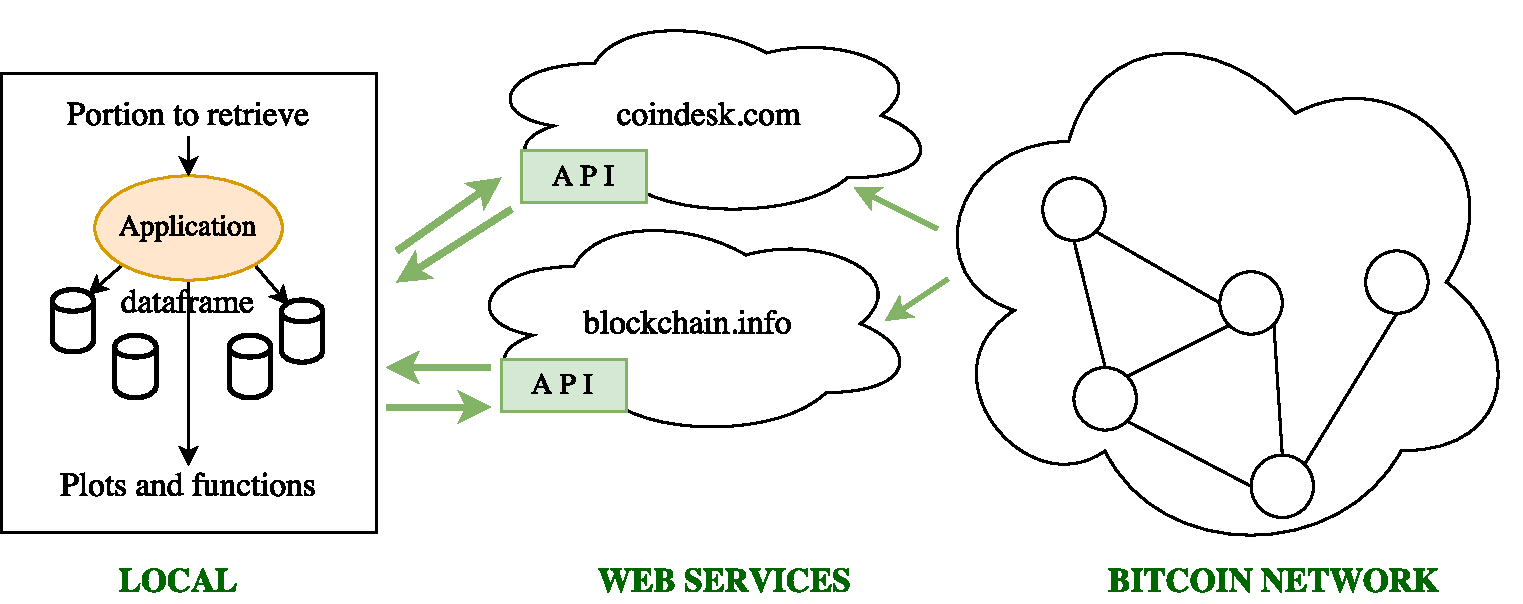
\includegraphics[width=1\textwidth]{img/architecture}
%	\caption{Architecture of the developed system for blockchain analysis.}
%	\label{fig:architecture}
%\end{figure}
%
%The architecture of our blockchain analytic system is showed in Figure~\ref{fig:architecture}. The system 
%is run mainly locally, importing Bitcoin \gls{api} and using them for data retrieval to the
%local system. The website \url{blockchain.info} provides \gls{api} to be used remotely with an
%HTTP request, and they can be easily integrated in the application with a HTTP
%request/response mechanism. The website \url{blockchain.info} contains all the information
%concerning the Bitcoin blockchain and it could be queried both through Python \gls{api}
%and web \gls{api}. This website is monitoring 24-7 the blockchain, producing graphs and
%statistical analysis on the data observed in the real decentralized network. The local
%application is monitoring these data as well, producing graphs that are not taken into
%consideration from the \url{blockchain.info} website, using a finer granularity that represent
%the data. Moreover, the application generates three text files:
%\begin{description}
%	\item [blockchain.txt:] text file containing information about the portion
%	of the blockchain retrieved, including block hash, height, size, fee and
%	time for each block. These data are important for the later analysis and the file is structured like the following:
%	\begin{lstlisting}
%hash:		block_hash
%epoch:		block_epoch
%creation_time: 	time_mining_block (s)
%size: 		block_size (byte)
%fee: 		block_fee (satoshi)
%height: 	block_height (block_number)
%bandwidth: 	read_bandwidth (MB/s)
%transactions: 	number_transactions_in_block
%avgttime: 	avg_tr_time (s)
%	\end{lstlisting}
%	\item [mining\_nodes.txt:] text file containing all the IP addresses of mining nodes or pools
%	concerning the blocks in the file "blockchain.txt".
%	\item [nodes\_in\_the\_network.txt:] text file containing all the IP addresses involved in relaying transactions
%	in the network.
%\end{description}
%
%The application for blockchain analysis is implemented in the file  \emph{observ.py}, it provides
%to call \gls{api} functions and to generates all the output files. A small
%example of how the \gls{api} calls work in the system is showed in Appendix~\ref{lst:api-python}.
%Our blockchain analytic system was implemented on a MacBook Pro with MacOS Sierra \emph{v$10.12.1$},
%with a $2.8$\,GHz Intel Core i$7$ processor and $16$\,GB~$1600$\,MHz DDR3 of RAM, using
%JetBrains PyCharm (\emph{v$2016.2.3$}) software as text editor and \emph{Python v$2.7.12$}
%as programming language.

\subsection{Data Retrieval}
\label{sec:data_retrieval}

%TODO: Show a table that list how data where retrieved, from where and why: SOURCE - ENTITY - INFORMATION table
%Data in the blockchain can be retrieved in different ways: blocks can be added to
%the top of the file, so the most recent blocks are fetched, or appended to the last element,
%so the blockchain is analyzed even further in the past.
%To fetch the most recent block the method showed in Appendix~\ref{lst:api-python}
%is used. First, the latest block is fetched, then from the previous is retrieved and so on.
%The latest block is saved with a structure showed in Appendix~\ref{lst:latest-block}.
%When data are appended to the last block, instead, is necessary first to get the hash
%from the last element in the "blockchain.txt" file, then the last block is retrieved
%using the method \emph{get\_block(hash)} provided from the Bitcoin \gls{api}.
%The implementation of the append is found in Appendix~\ref{lst:append-block}.
%
%Blockchain is meant to be ordered linearly and every block should have its predecessor,
%for this reason blocks are collected in a way that there will not be any gap in the local blockchain, and
%if the number of blocks that the user tries to fetch is less than the blocks
%already added to the global blockchain, then would be impossible to add any new block.
%In this case a better option would be to \emph{update} the local blockchain (-u command, view the application
%usage~Appendix~\ref{lst:usage}), which means that the right number of blocks that will complete
%the local chain will be automatically retrieved. A simplified scheme to add blocks on
%the local blockchain is showed in Figure~\ref{fig:blockchain-scheme}. To guarantee that the order is
%respected and the blockchain is saved locally in a correct way, a validity check is done every time
%the application is executed. This check verifies that
%each block in the local blockchain has the right predecessor by controlling that there is a
%diminishingly height by one going from one block to another (Appendix~\ref{lst:check}).
%\begin{figure}[h!]
%	\centering
%	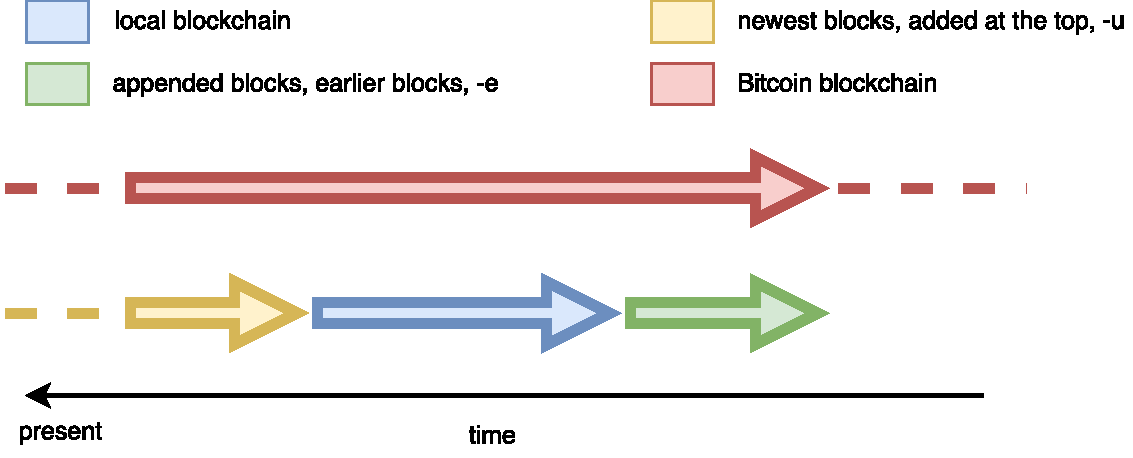
\includegraphics[width=1\textwidth]{img/blockchain-scheme}
%	\caption{Scheme that shows how blocks are written in the local blockchain file.}
%	\label{fig:blockchain-scheme}
%\end{figure}
%
%Once blocks are retrieved a \emph{file.write} is performed. Writing on blockchain.txt
%can be done by appending blocks at the end or adding them at the beginning
%of the file. As Appendix~\ref{lst:file-write} shows, the adding part is much more
%complicated since the file needs to be deleted and then written again for each block
%that needs to be added.
%As showed in Chapter~\ref{sec:implementation} before plotting and getting any
%kind of information from the data, they are evaluated and manipulated for our purposes.
%The blockchain.txt file saved, contains information about block hash, height, size, fee, epoch
%time, creation time, read bandwidth, number of transactions and the average transaction
%visibility time (average write bandwidth for a block). Of course not all these data are
%provided from the Bitcoin \gls{api}, so they are calculated and manipulated runtime, then saved in the text file.

\subsection{Data Manipulations}
%Data manipulation is done both before (to save data correctly) and after
%(to plot data correctly) data are collected in the
%blockchain.txt file. Once data are retrieved and saved, they are ready to
%be manipulated in a way that the right and needed information can get
%out of them.
%
%Each block $B$, retrieved from the blockchain.txt file, has the following attributes.
%The \emph{hash}, $B.hash$, is a string containing the 256-bit hash for the block $B$.
%The \emph{epoch}, $B.epoch$, which represents the epoch time when the block was created and
%got visible in the blockchain. This means that the retrieval time is in seconds,
%starting from the epoch which is $1^{st}$ January $1970$ at $00$:$00$:$00$. The time is
%always collected as seconds and if needed, is converted in minutes and
%hours and saved in other lists.
%The \emph{size}, $B.size$, is represented in bytes, so every time that MB are needed, the
%size is divided by $10^6$. The growth of the blockchain is represented in GB and
%the block size and the read/write bandwidth in MB.
%The \emph{fee}, $B.fee$, represents how much the miner of the block get in satoshi~(Appendix~\ref{app:terminology})
%to mine a certain block $B$. To be more readable, plots using satoshi are converted in BTC.
%The \emph{creation time}, $B.creation\_time$, is represented in seconds, and it tells how much time
%a block needs to be mined.
%The \emph{number of transactions}, $B.transactions$, tells how many transactions are accepted and
%stored in the block $B$.
%The \emph{write bandwidth}, $B.avgttime$, is the average of the all transactions acceptance time
%in a certain block and it is measured in seconds. A transaction $T$ is accepted when the block $B$ is
%created so the $read\_bandwidth_T$ will be:
%\begin{equation}
%\label{eq:read_bandwidth}
%read\_bandwidth_T = B.epoch - T.time
%\end{equation}
%where $T.time$ is the epoch representing the transaction request.
%
%The read bandwidth is calculated as showed in Appendix~\ref{lst:read-bandwidth}.
%Start time and end time are calculated before and after the block retrieval call, with
%the function \lstinline|datetime.now()|. Time is manipulated to be showed in seconds and then
%the ratio to get the bandwidth between $MB/s$ is done and the value is appended
%in a list that will be written in the file.
%
%The write bandwidth is calculated first for each transaction in the block, as the
%Appendix~\ref{lst:get-transaction-time} shows, and then an average is done
%for each block and returned as a data to append in a list containing
%all the write bandwidths for each block retrieved, this data is written in the
%blockchain.txt file as \emph{avgttime}.
%
%To represent the growth of the blockchain, a growing time and size list needs
%to be generated. Assuming that a block is represented with $B$ and its creation time is $B.epoch$,
%we define the block creation time in the following way:
%\begin{flalign}
%\label{eq:creation_time}
%creation\_time_n = \begin{cases} 0, & \mbox{if } n = 0\\ B.epoch_n - B.epoch_{n-1}, & \mbox{if } n > 0 \end{cases}&&
%\end{flalign}
%where $B.time_{n-1}$ is its predecessor.
%The growth of the blockchain is calculated by comparing the sum of the creation time
%and the sum of the block size each time, generating ever growing lists as shows the Appendix~\ref{lst:growing-lists}.
%Assuming that $B.size$ is the block size, then:
%\begin{flalign}
%\label{eq:growing_time}
%&growing\_time_n = \begin{cases} 0, & \mbox{if } n = 0\\ creation\_time_n + creation\_time_{n-1}, & \mbox{if } n > 0 \end{cases}&&
%\end{flalign}
%and:
%\begin{flalign}
%\label{eq:growing_size}
%&growing\_size_n = \begin{cases} 0, & \mbox{if } n = 0\\ B.size_n + B.size_{n-1}, & \mbox{if } n > 0 \end{cases}&&
%\end{flalign}
%where $growing\_time$ is the list containing the sums of the creation time every time that a new
%block is created and $growing\_size$ is the list containing the size of the blockchain
%as every block is added.
%
%One of the reason why Python was chosen as a programming language is because
%data structures are easy to manage and with a Python list you can change the whole
%data in it using only one line of code~(Appendix~\ref{lst:python-list}). It is very easy indeed to swap an entire
%list from minutes to seconds, from seconds to hours and vice versa. Furthermore,
%mature API bindings do exist for Python, and it is a very intuitive language with a lot
%of useful libraries for data manipulation and plotting.

\subsection{Methods}
%TODO: Define formulas
%$t_l = B_{epoch} - t_{epoch}$


%An UML diagram of the main methods used in the application is represented in
%Figure~\ref{fig:uml_sequence_diagram_application}.
%The application usage is described in Appendix~\ref{lst:usage} and the main
%methods in the systems are:
%\begin{description}
%	\item [\emph{get\_blockchain(n, [hash])}:] method that retrieve the blocks
%	from the Bitcoin blockchain and saves them in lists that will be the input
%	of the write\_blockchain() method. If the attribute hash exists then the retrieval
%	starts from that hash and not from the latest block created in the Bitcoin blockchain.
%	Part of it is represented in Appendix~\ref{lst:append-block}.
%	\item [\emph{write\_blockchain(<lists to write>, [to\_append])}:] method that takes lists in input and write them into a file,
%	according to the parameters that it gets. If to\_append is True, then data are appended otherwise are added, like
%	shows Appendix~\ref{lst:file-write}.
%	\item [\emph{get\_list\_from\_file(attr)}:] this method is probably one of the most important concerning data
%	manipulation. It creates a list, given an attribute as input. Such attribute is a block information stored in the
%	local blockchain and the list generated contains all the values from every block, concerning that
%	particular  attribute.
%	Lets say that informations about the block hash want to be analyzed, then it would only be necessary
%	to make a call to this method giving as attribute the string \emph{"hash"}, like showed in Appendix~\ref{lst:get-data-from-file}.
%	In that way the return list will contain hashes about all the blocks retrieved with the most recent hash In list[$0$].
%	Regular expression\,\cite{Aho:1992:FCS} is used to analyze the file and read from it, in this way is possible
%	to interact with the saved data and get informations from them. This method allows the
%	function plot\_data() to easily display statistics.
%	\item [\emph{plot\_data(d, n, [r], [s], [e])}:] this method gets the data from the
%	txt file and then plots all the information retrieved using Matplotlib libraries\,\cite{matplotlib}. It has
%	a description, $d$, a number of the plot, $n$, and an optional parameter about the
%	regression, $r$. It also has the possibility to chose the range of the plot with the start, $s$, and end, $e$,
%	parameters. If in the local txt file are present $10000$ blocks, is possible to call the method with
%	$start=7000$ and $end=9000$, in that way only the blocks in between $7000$ and $9000$
%	will be taken into consideration for the plots. In that way is easier to verify if the predictions on
%	the blockchain growth were accurate or not.
%\end{description}
%
%\begin{figure}[h]
%	\centering
%	\begin{sequencediagram}
%		\newthread{m}{main()}
%		\newinst{gb}{get\_bc()**}
%		\newinst{wb}{write\_bc()**}
%		\newinst{bi}{bc.info**}
%		\newinst{pb}{plot\_data()*}
%		
%		\begin{callanother}{m}{1}{gb}{}
%			\mess{gb}{}{bi}
%			\mess{bi}{get data}{gb}
%				\begin{callanother}
%				{gb}{2}{wb}{}
%			\end{callanother}
%		\end{callanother}
%
%		\begin{callanother}
%			{m}{3}{pb}{}
%		\end{callanother}
%		
%	\end{sequencediagram}
%	\begin{enumerate}
%		\item call the method \emph{get\_blockchain()} for blocks retrieval
%		\item write data in the txt.file
%		\item call the plot function for data plotting
%		\item[*] not every function or method is showed in the diagram, the
%		function plot\_data() calls some methods for data management.
%		\item[**] the word blockchain has been replaced with the shortcut
%		bc
%	\end{enumerate}
%	\caption{UML sequence diagram of how the application works, where
%		the threads are the methods implemented in \emph{observ.py} file.}
%	\label{fig:uml_sequence_diagram_application}
%\end{figure}
%
%
%The \emph{main()} method provides to call the others and if the
%\gls{grasp} principle is followed\,\cite{Larman:2004:AUP}, then this method would be
%the controller, dispatching calls to other methods for collecting, analyzing and plotting
%data.
%
%Not all the methods implemented in the system are listed above. Some include
%data management or check of the blockchain status, such as converting the
%epoch time in date time format $DDMMYYYY$, get the number of blocks currently
%present in the local blockchain or create the growing size and time lists.
%The method \emph{add\_mining\_nodes(block)} concerns the creation of a file containing
%mining nodes and a file containing nodes involved in every transaction. The second
%one are the nodes that rely transactions in all the block retrieved.
%This means that for each block given in input, every transaction is analyzed, and if the node
%relying this single transaction is not in the file yet, then the IP for this node is added to it.

\section{Version Control}
\label{sec:versioncontrol}
%For the version control on the source code, a public \emph{git} repository at:
%\url{https://github.com/ted92/blockchain.git} was created. Git version \emph{2.6.4}
%is used in the local environment and every significant update is pushed to the
%repository to keep an history of all the changes and how the application was
%developed.

\chapter{Blockchain Observations}
\label{chap:evaluation}
%TODO: Our observations could be miners oriented or epoch oriented. Analyzing categorical data such as mining pools we could determine which ones are more effective than others and why a block should most likely be mined by a certain mining pool rather than another. Studying the epoch instead, gave us useful informations about the changes and the development of the blockchain during time.

%TODO: In our studies, we focused on finding any correlation between attributes using heat map with \emph{seaborn}\,\cite{michael_waskom_seaborn}. If the heat map chart shows any possible correlation then we study the degree of correlation between two attributes, $corr(u,v)$, which can be quantified using Pearson's correlation coefficient showed in Eq.\,\ref{eq:pearson}. However, calculating the correlations and printing them or drawing cross-plots works fine for few correlations, but it is difficult to get a grasp of a large table of numbers, and it is difficult to squeeze all the cross plots onto a page if the problem has a large number of attributes. For that reason we use a heat map with Pearson's correlation coefficient for pairs of attributes arranged into a matrix where the $m_{ij}$ entry is the correlation between the $i^{th}$ attribute and the $j^{th}$ attribute.

%TODO: The next step wants to get some ideas about the relationship among the attributes and between attributes and labels including also categorical attributes.

%TODO: We used for prediction both, \emph{linear} and \emph{nonlinear} algorithms and we considered that linear models are preferable when the data set has more columns than rows or when the underlying problem is simple, nonlinear models are preferable for complex problems with many more rows than columns of data.

%TODO: To get values in $(0,1)$ the logit function in Eq.\,\ref{eq:logit} is applied to our data.


%TODO: The Bitcoin price has been affected of an high volatility. For that reason, predicting the fee in \gls{usd} that a client might pay is difficult and it might change from the Bitcoin price. According to \emph{Coindesk.com}.... show the bitcoin price!

%TODO: Block size limit can set the number of transactions the network can confirm per block, so the throughput of the whole Bitcoin network.

%TODO: In our longitudinal plot each data point visualizes aggregated data of \# blocks.
%In this chapter we present observations of the Bitcoin blockchain captured by the
%analytics system outlined in Chapter~\ref{chap:expsetup}. 
%To evaluate our problem definition in Chapter~\ref{sec:probdefinition}, we focus on consideration related to 
%read/write bandwidth, the growth of the blockchain, and the relation between the fee paid and the bandwidth achieved.
%The evaluations are made by analyzing the plots generated in the plot/
%folder using Matplotlib\,\cite{matplotlib}. A large number of test has been
%done, considering always a different number of blocks fetched, at different time.
%%TODO: put the following also in the abstract and in the introduction
%We show that the fee paid is related to the amount of time that a block needs to be mined and be visible in the whole network.
%This affects average bandwidth available to an application.

\section{Blockchain Growth}
\label{sec:blockchain_growth}
%To understand the capacity of the Bitcoin blockchain, we first study
%its size and how it grows over time. For this, we've been analyzing the blockchain
%periodically from the $21^{st}$~September~$2016$ until the $11^{th}$~December~$2016$
%using the system outlined in Chapter~\ref{chap:expsetup}. The plotted growth is
%shown in Figure~\ref{fig:growth_blockchain}. We observe that the blockchain size grows
%of $10,139$\,GB in $1940$ hours. That means a bandwidth usage of $\sim5,22$\,MB per hour. 
%Our findings are inconsistent with the observations from
%$2014$~\cite{ethereum_white_paper} that observed a growth
%of~$\sim$1\,MB per hour. Our observations indicate that the growth of the
%Bitcoin blockchain is $5x$ times bigger than it was expected in 2014 and we
%believe that a more accurate model for the blockchain growth can be created.

%\begin{figure}[h!]
%	\centering
%	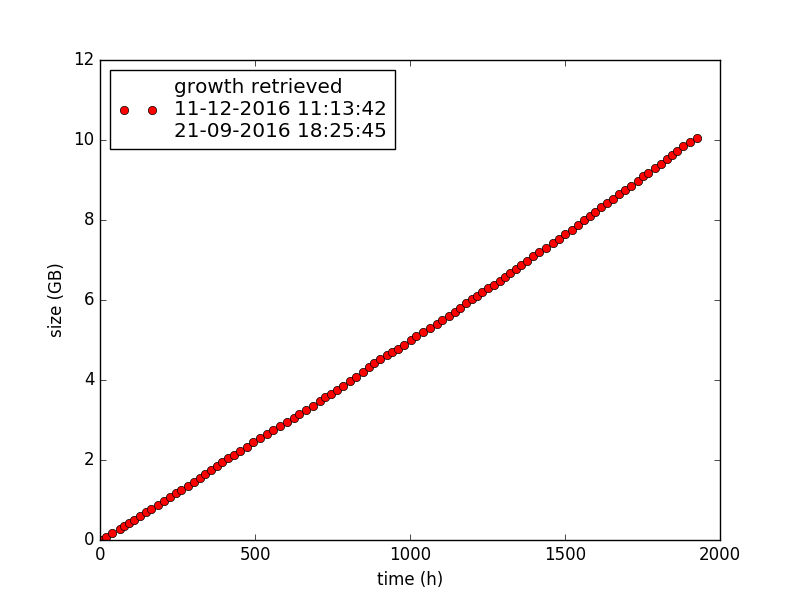
\includegraphics[width=1\textwidth]{img/growth_blockchain}
%	\caption{The Bitocin blockchain growth according to our analytics system.
%		12091 blocks are fetched between the $21^{st}$~September~$2016$ and the $11^{th}$~December~$2016$.}
%	\label{fig:growth_blockchain}
%\end{figure}

%From the plot in Figure~\ref{fig:growth_blockchain} the growth seems to be linear.
%However, evaluations made using polynomial interpolation on these data show that the growth has,
%even if small, a coefficient on the $x^2$. Our hypothesis is that the non-linear growth
%is due to a small increment of the block size during the years.
%To prove this, two different measurements have been done to our local blockchain, showed in
%Figure~\ref{fig:size_comparison}. The first one, Figure~\ref{fig:size_comparisonA},
%considers $1000$ blocks fetched from $22^{nd}$~September~$2016$ until
%$28^{th}$~September~$2016$, shows that the block size tends to be $1$\,MB
%but with quite a lot of blocks having also different sizes. While the latest one, in Figure~\ref{fig:size_comparisonB},
%shows that almost every block out of $1000$ are tending to the $\sim1$\,MB size, having only few blocks under
%the $1$\,MB "line". The second measurement was evaluated between $04^{th}$~December~$2016$ and
%$11^{th}$~December~$2016$.
%Furthermore, if the blocks from $2009$ in the blockchain are analyzed, their sizes tend
%to be~$\sim$200\,kB while in this last months of analysis, December~$2016$ the block size tend to be of $\sim1$\,MB.
%This brings us to believe that the average block size is growing with time,
%hence the blockchain growth is not linear as previously claimed\,\cite{ethereum_white_paper}. 

%\begin{figure}[H]
%	\centering
%	\begin{subfigure}{1\textwidth}
%		\centering
%		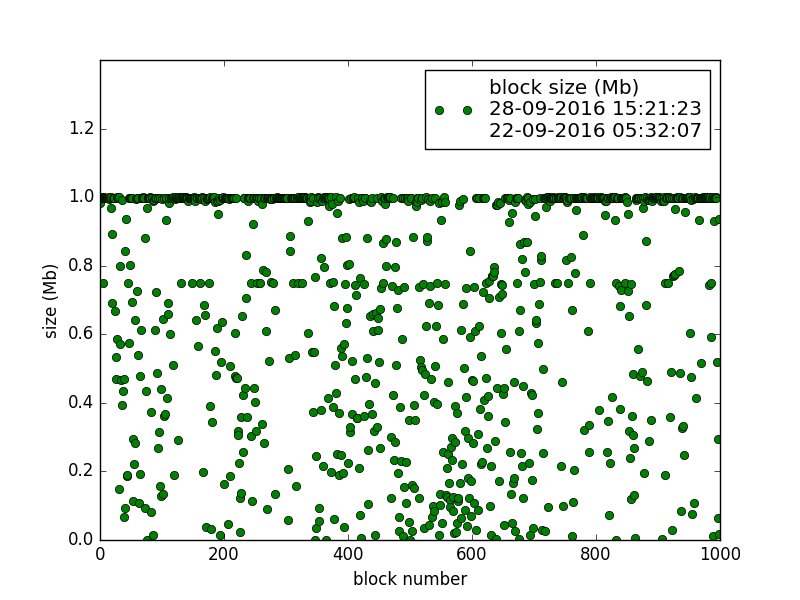
\includegraphics[width=1\linewidth]{img/byte_per_blockA}
%		\caption{Late September~$2016$.}
%		\label{fig:size_comparisonA}
%	\end{subfigure}
%
%	\begin{subfigure}{1\textwidth}
%		\centering
%		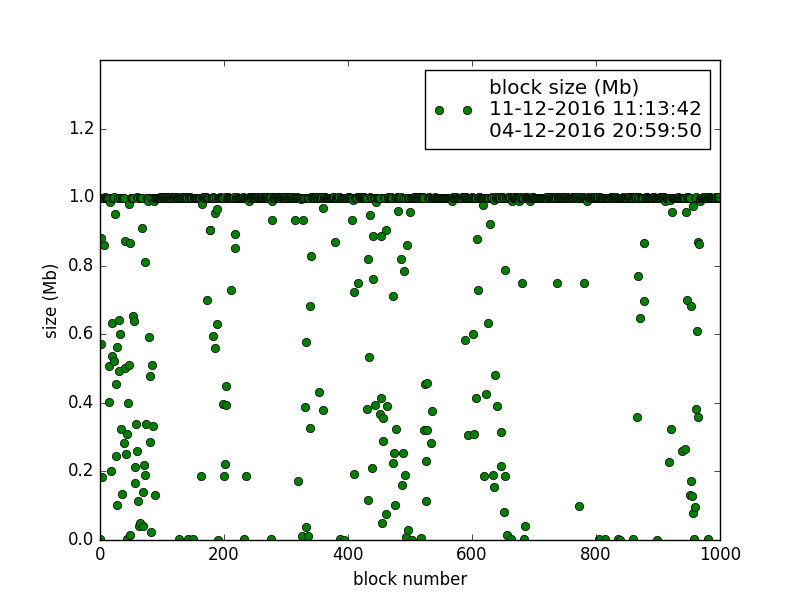
\includegraphics[width=1\linewidth]{img/byte_per_blockB}
%		\caption{Mid December~$2016$.}
%		\label{fig:size_comparisonB}
%	\end{subfigure}
%	\caption{Size comparison of $1000$ blocks with more than 2 months of gap.}
%	\label{fig:size_comparison}
%\end{figure}

\section{Retrieval Block Time}
%\label{sec:retrieval_block_time}
%The biggest problem analyzing the blockchain was that the \gls{api} allows to
%retrieve only one block per time, making the block fetching incredibly slow. This
%is the reason why the block retrieval is kept separate from the analytics part,
%in that way is possible to fetch a fewer number of blocks, adding them time
%by time and at the end make analysis on them.
%In Figure~\ref{fig:bandwidth} the read bandwidth for each block retrieval is
%represented. As said before, the problem of a single-block-fetch affects
%drastically the latency, and then the read bandwidth as well,
%taking an average of~$\sim1$\,seconds to retrieve a
%single block, and in some blocks the read bandwidth is even less than $0,5$\,MB/s.

\section{Block Analysis}
\label{sec:block_analysis}
%The most important attributes of blocks are their size, their creation times, and the
%number of transaction in each individual block. In this section, we will compare this
%three attributes to see if there could be any relation between them.
%The plot in Figure~\ref{fig:efficiency} shows that the block size tend to be $\sim1$\,MB.
%This observation does not depend on how many
%transactions it contains or how much time it needed to be mined.
%No relation also was found between the number of transactions in a block and the block
%creation time. In the Figure~\ref{fig:efficiency} sometimes the blue line (block creation time)
%follows the red one (number of transactions in one block), so if one grows then also the
%other gets higher, but in other cases there is a reverse dependence, so if the number of
%transactions grows, the block creation time decreases. This unpredictability
%is good for the security of the blockchain, since malicious node cannot find any dependence
%on the data which are more representative for a block.
%
%Figure~\ref{fig:time_per_block} shows the creation time for each block,
%retrieving blocks from the Bitcoin blockchain between the $4^{th}$
%and $12^{th}$~December~$2016$. How mining works is described in
%Chapter~\ref{sec:mining} and according to the difficulty, which is constantly adjusted, a
%block should be mined every $10$\,minutes\,\cite{bitcoinmining}. This claim
%tend to be verified for most of the blocks, however, there are too many peaks with a
%creation time of $20$\,minutes (which is already the double) until $40$\,minutes, up to even
%$80$\,minutes per block. When a block takes $80$\,minutes to be mined, it will affect the
%visibility of all the transactions in that block, mining the consistency of the system, since, in
%an average scenario a sender expects that its transaction is visible after $\sim8$-$15$\,minutes.
%\begin{figure}[h]
%	\centering
%	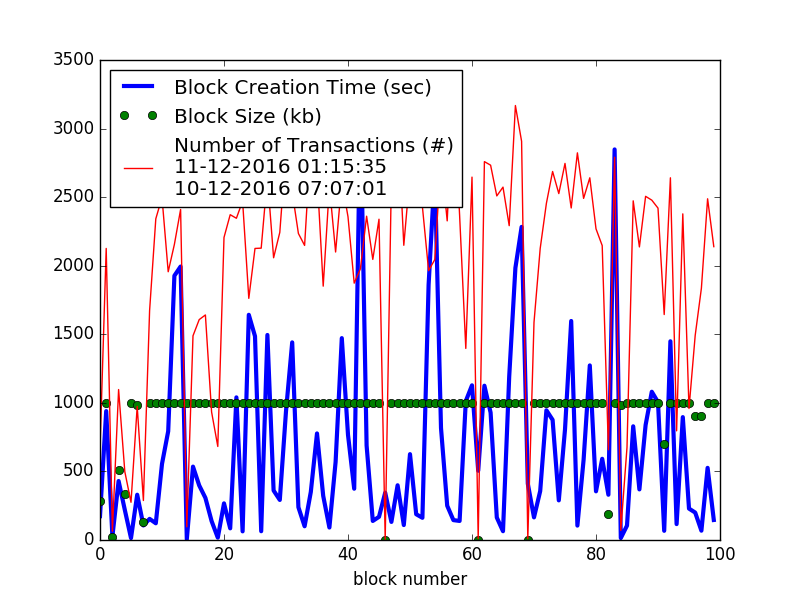
\includegraphics[width=1\textwidth]{img/efficiency(100)}
%	\caption{Relation between block creation, block size and number
%		of transaction in a block. Measurement done on
%		Bitcoin blockchain from $10^{th}$~December~$2016$ until
%		$11^{th}$~December~$2016$.}
%	\label{fig:efficiency}
%\end{figure}

\section{Bandwidth}
\label{sec:bandwidth}
%As explained in Chapter~\ref{sec:method}, the bandwidth represents the speed,
%in MB/s, for a transaction to be visible and accepted (write bandwidth), and the speed, always in MB/s, that
%a node has while fetching this block (read bandwidth). The Figure~\ref{fig:bandwidth}
%shows that the read bandwidth while monitoring the blockchain for more than 2 months,
%has an average speed of $\sim1$\,MB/s and it doesn't go faster than $9$\,MB/s. This
%makes the read bandwidth quite slow, not allowing us to fetch as many blocks as we want
%per time. An average block fetching time is~$\sim1$\,second,
%having then a total computation time, while fetching $2000$ blocks, of~$\sim40$\,minutes.
%Furthermore, some \gls{api} errors like "Connection reset by peer" or "Maximum concurrent
%requests for this endpoint reached" occurred. That leads our system development to
%allow the block retrieval with small number of blocks, and then append them in a text file,
%as explained in Chapter~\ref{chap:expsetup}.
%
%\begin{figure}[h]
%	\centering
%	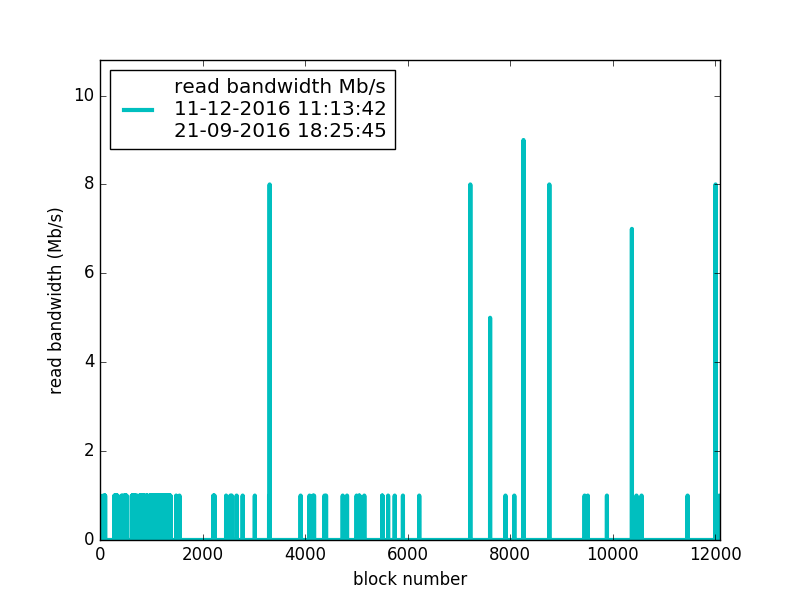
\includegraphics[width=0.9\textwidth]{img/bandwidth}
%	\caption{Read bandwidth of the Bitcoin blockchain measured according to
%		the size of the block fetched and the time taken to fetch that block.
%		Measurement done Measurement done from $21^{st}$~September~$2016$ until
%		$11^{th}$~December~$2016$.}
%	\label{fig:bandwidth}
%\end{figure}

%In Figure~\ref{fig:comparison_visibility_blockcreation} is represented the comparison between
%the block creation time, Figure~\ref{fig:time_per_block}, the average visibility time for
%transactions in each block,
%Figure~\ref{fig:transaction_visibility}, and the the transaction
%visibility provided from the Bitcoin website, Figure~\ref{fig:transaction_visibility_bitcoinwebsite}.
%The comparison was made using exactly the same
%blocks, retrieved from $4^{th}$ until $12^{th}$~December~$2016$. The first thing to notice is that,
%despite the block creation time is never higher than $80$\,minutes, is that there are some
%transactions
%that take more than $1$\,day to be visible. This because miners gives the priority to transactions that are
%willing to pay an higher fee. A lot of transactions are not paying any fee, so they
%will not be included immediately to the next block creation. This thing was not very well explained anywhere
%and it was clear only after this data analysis.
%
%The plot from \url{blockchain.info} in Figure~\ref{fig:transaction_visibility_bitcoinwebsite} shows that,
%in one month, the average confirmation time is~$\sim10$\,minutes, with a peak of $16$.
%Considering though a finer granularity, in about a week of transactions, as shows Figure~\ref{fig:transaction_visibility},
%there is yes a coarse median of~$\sim10$-$20$ minutes, but there are a lot $40$ minutes peaks, some peaks
%of $300$ and $400$ minutes and even others of $1000$ and $1900$ minutes.
%This data might be relevant for a big company who decides to invest a lot in Bitcoin, then
%they need to know that a transaction could take even $100x$ time than what is showed
%in the Bitcoin website.
%
%\begin{figure}[H]
%		\centering
%	\begin{subfigure}{.7\textwidth}
%		\centering
%		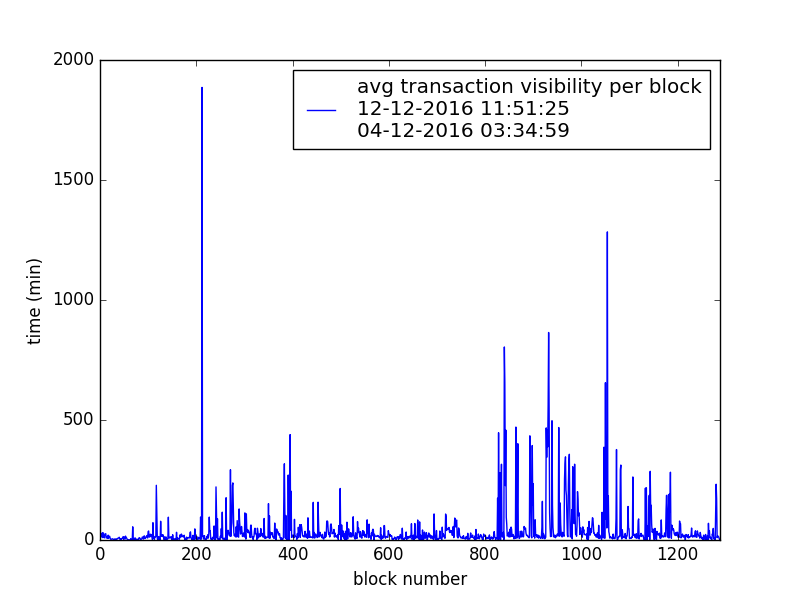
\includegraphics[width=1\linewidth]{img/transaction_visibility}
%		\caption{Average time for a transaction to be visible in the public ledger since
%			its first creation request.
%			Measurement done between $4^{th}$ and $12^{th}$~December~$2016$ on the
%			Bitcoin blockchain.}
%		\label{fig:transaction_visibility}
%	\end{subfigure}%
%
%	\begin{subfigure}{.7\textwidth}
%		\centering
%	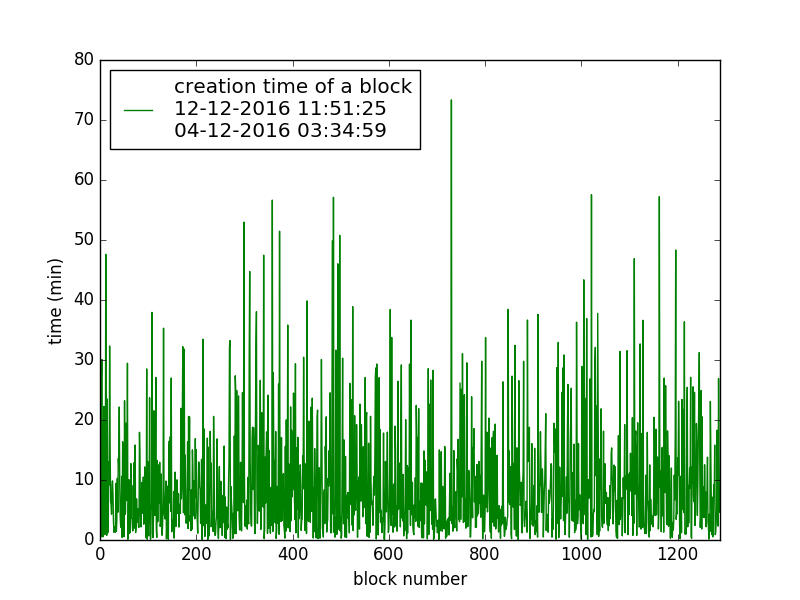
\includegraphics[width=1\textwidth]{img/time_per_block}
%	\caption{The block's creation time in the Bitcoin blockchain. Every block is
%		created each $m$ minutes. Data from $4^{th}$ until $12^{th}$~December~$2016$ are
%		considered for this test.}
%	\label{fig:time_per_block}
%	\end{subfigure}
%	
%	\begin{subfigure}{.7\textwidth}
%			\centering
%		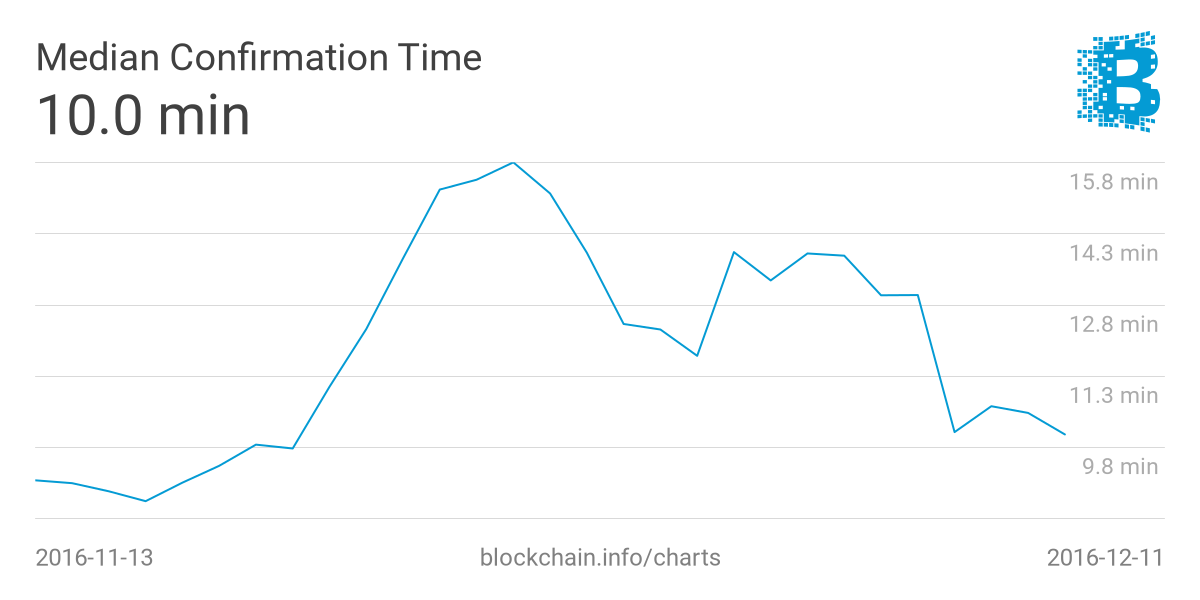
\includegraphics[width=1\textwidth]{img/transaction_visibility_bitcoinwebsite}
%		\caption{Median confirmation time for a transaction. Data from the official Bitcoin website
%			\url{blockchain.info} \cite{bitcoin_blockchain}.}
%		\label{fig:transaction_visibility_bitcoinwebsite}
%	\end{subfigure}
%	\caption{Comparison between block size and the average time for a transaction to be visible in the public ledger.}
%	\label{fig:comparison_visibility_blockcreation}
%\end{figure}

\section{Block Fee}
\label{sec:block-fee}
%In this thesis we aim to find a relation between
%the fee paid to the miner and the block creation time. Before, we saw
%that more a client is willing to pay for a transaction fee ($T_g$) more are
%the probability that its transaction is included immediately in the next block.
%Here we want to confirm the relation that exists between the creation time
%and the fee paid to the miner. In Figure~\ref{fig:fee_bandwidth} an analysis
%between the $21^{st}$~September~$2016$ and the $12^{th}$~December~$2016$
%is done, retrieving $12100$ blocks, and it is pretty clear that there is a certain
%relation between the series of data analyzed. This confirms that,
%more computational effort is put into a block creation and more fee
%is paid to the miner or pool of miners who solve the proof of work.
%Of course there are occasional exceptions, if a block contains a lot of transaction
%with $T_g$ equal to zero, the fee paid to the miner will be lower if compared to
%the one given from a block containing only high priority transactions, which is extremely unfair.
%This is why current, decentralized digital currencies are trying to avoid transactions
%with $T_g$ equal to zero by ignoring them. On the other hand the Figure~\ref{fig:fee_bandwidth}
%shows that there are only couple of blocks that take high computational time, $\sim35$-$38$\,minutes, and get
%a low reward, almost $0$\,\gls{btc}.
%\begin{figure}[H]
%	\centering
%	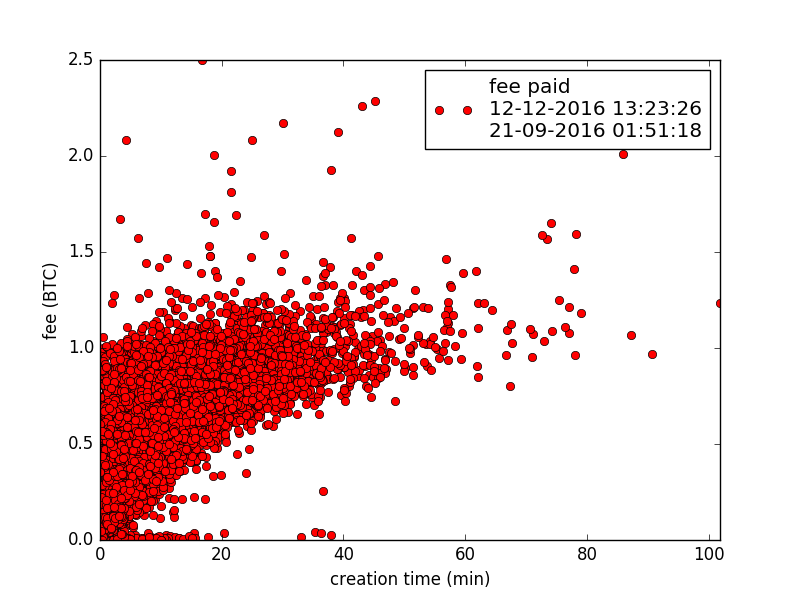
\includegraphics[width=1\textwidth]{img/fee_bandwidth}
%	\caption{Relation between the fee paid to the miner and the block creation time.
%		Measurement done on the Bitcoin blockchain between
%		the $21^{st}$~September~$2016$ and the $12^{th}$~December~$2016$.}
%	\label{fig:fee_bandwidth}
%\end{figure}
%With this observation, it becomes possible to generate a model that,
%in future implementation, could help blocks to get the expected reward for mining. The model
%created is showed in Chapter~\ref{sec:models} and it is generated with the
%polynomial interpolation of the data in Figure~\ref{fig:fee_bandwidth}.

\section{Models}
\label{sec:models}

%Next, we generate a model
%that predict the future growth of the blockchain and help nodes to smartly use their bandwidth.
%To get the model for the blockchain growth, data are collected and then a statistical
%regression is made on them. The function that represents the blockchain growth is obtained
%thanks to the \emph{NumPy} libraries\,\cite{scipy}. To find the model that more fits our data, polynomial
%interpolation was applied\,\cite{Hildebrand:1987:INA}. An example of the code regarding it is found
%in Appendix~\ref{lst:polynomial-interpolation}.

%\begin{figure}[H]
%	\centering
%	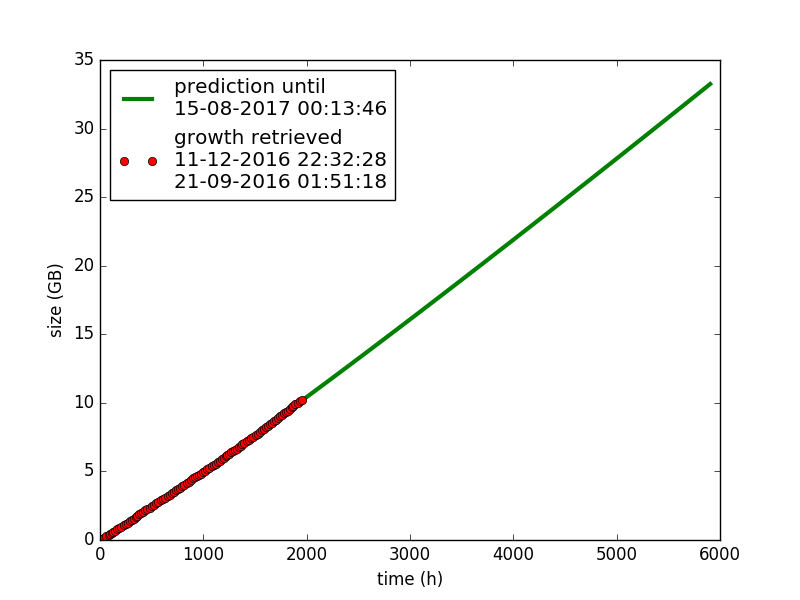
\includegraphics[width=1\textwidth]{img/regression_growth_blockchain}
%	\caption{Regression of the growth of the blockchain with a prediction model.
%		Measurement done on the
%		Bitcoin blockchain between the $21^{st}$~September~$2016$ and the
%		$11^{th}$~December~$2016$.}
%	\label{fig:regression_growth}
%\end{figure}

%Considering the blockchain growth, a prediction of $3x$ time in the future has been evaluated. If
%the evaluation is done considering $1000$\,blocks, with a total time of $150$\,hours, then the
%prediction will be on how much the blockchain will grow in the following $300$\,hours.
%The Figure~\ref{fig:regression_growth} shows that the blockchain, as expected, has an
%almost linear growth. It has though a very little quadratic coefficient due to the
%slightly increment of the block size among the years. The function evaluated using the polynomial
%interpolation for the blockchain growth is the following:
%\begin{equation}
%\label{eq:growth_regression}
%f_g(x) = \frac{9}{10^8}x^2 + \frac{5}{10^{3}}x
%\end{equation}
%According to the prediction in Figure~\ref{fig:regression_growth}, analyzing data
%from $21^{st}$~September until $11^{th}$~December~$2016$, the blockchain
%will grow of $\sim28$\,GB by August~$2017$.
%To verify the veracity of this prediction, we applied this method from September~$2016$
%to December~$2016$ so that we have the real growth to compare. Even though the data
%used were not so many ($2000$ blocks for $1$ month forecast compared to the $12200$\,blocks
%used in the Figure~\ref{fig:regression_growth}), they were accurate in the prediction.
%That model has told us that by the $14^{th}$ of December~$2016$ the blockchain was
%supposed to grow of $9,5$\,GB, when only data from September~$2016$
%were evaluated. The blockchain has grown with about $10$\,GB instead, but
%still, considering the few data analyzed, the model generated is accurate and reliable.
%More data are used for the prediction, more accurate will be the function generated.
%
%\begin{figure}[h]
%	\centering
%	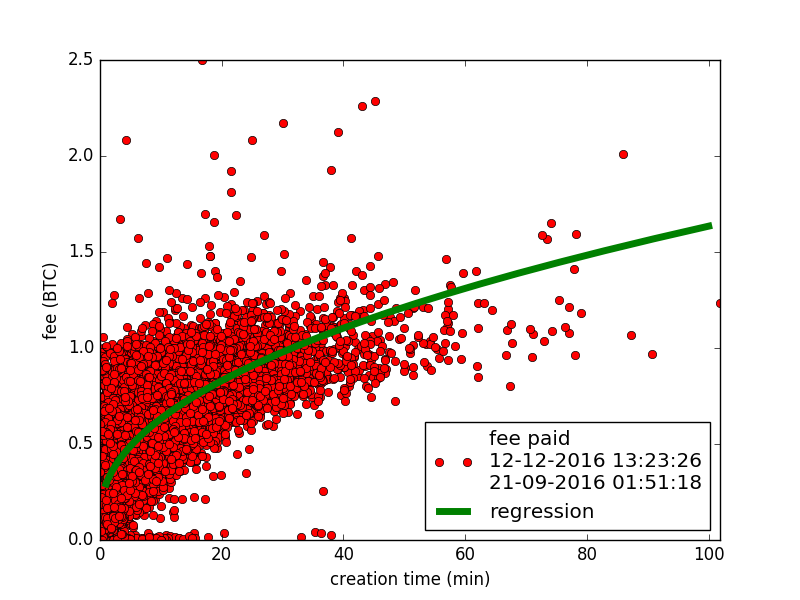
\includegraphics[width=1\textwidth]{img/fee_regression}
%	\caption{Regression of the relation between the fee paid
%		to the miner and the block creation time.
%		Measurement on the Bitcoin blockchain between
%		the $21^{st}$~September~$2016$ and
%		the $12^{th}$~December~$2016$.}
%	\label{fig:fee_regression}
%\end{figure}

%The Figure~\ref{fig:fee_regression} shows that there is a relation between the fee paid
%and the creation time of a block. This relation seems to be quadratic/logarithmic.
%The regression is found using NumPy libraries~\cite{scipy} and the function is obtained
%with the polynomial interpolation. More data are analyzed, more the function
%generated is accurate. The one showed below in (\ref{eq:fee_regression}) is created
%by collecting data from  $21^{st}$~September~$2016$ until $12^{th}$~December~$2016$. 
%\begin{equation}
%\label{eq:fee_regression}
%f_{Bg}(x) =  \begin{cases}-\frac{1}{10^4}x^2 + \frac{3}{10^2}x + 0,3 & \mbox{ with } x < 100 \end{cases}
%\end{equation}
%Note that this function is valid if the creation time, $x$, is
%lower than $100$\,minutes.
%This model could be useful for a miner which expects a certain fee after mining for \emph{n}
%minutes, to see if the fee they received is below or above the function model. In that way for the next
%mining processes a block will be in debit or credit and he will consider only transaction with an higher
%$T_g$, or transaction with a lower $T_g$ according of how much is its credit/debit.
%
%The last model generated is showed in Figure~\ref{fig:transaction_fee_bandwidth}. It
%represents the average approval time for the transactions in a block, compared to
%the fee paid ($B_g$) divided by the number of transactions in that particular block.
%Then for each block $B$ we calculated the average $T_p$, $\overline{T_p}$, as:
%\begin{equation}
%\label{eq:transaction_fee}
%\overline{T_p} = \frac{B_g}{|B_t|} 
%\end{equation}
%where $|B_t|$ is the number of transactions approved from the block $B$.
%The plot in Figure~\ref{fig:transaction_fee_bandwidth} shows that if a transaction
%pays from $0$ to $0.001$\,\gls{btc}, then the visibility would be almost random.
%However if their $T_g$ is increased from $0.002$ and $0.006$\,\gls{btc} their
%visibility will be seldom above $35$\,minutes and most likely between $5$ and $15$\,minutes.
%The function generated with the polynomial interpolation is the following:
%\begin{equation}
%\label{eq:transaction_fee_bandwidth}
%f_t(x) = \begin{cases}\frac{1}{10^8}x^2 - 5000x + 35 & \mbox{ with } x < 0.007\end{cases}
%\end{equation}
%The function showed in~(\ref{eq:transaction_fee_bandwidth}) is important
%for a transaction that needs a certain bandwidth, in a way that it knows, approximately, how much
%$T_g$ should be willing to pay according to get a positive bandwidth.
%
%\begin{figure}[h]
%	\centering
%	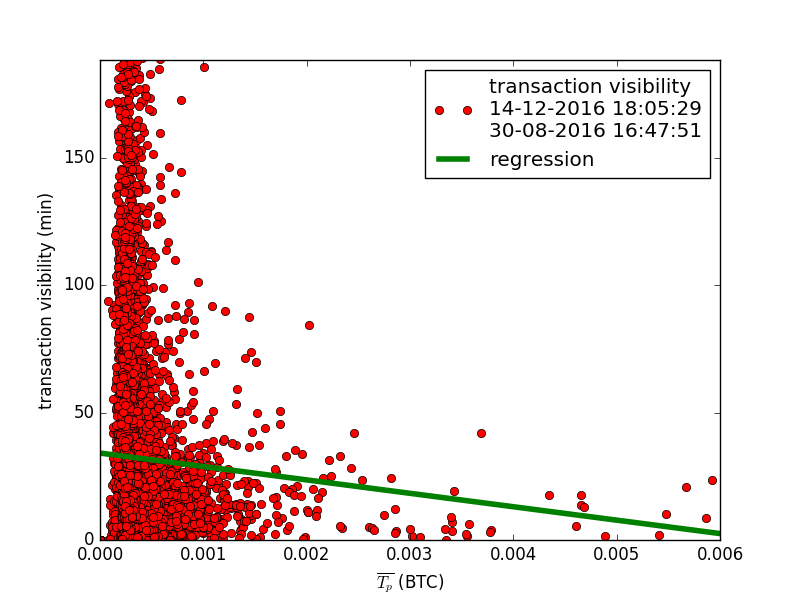
\includegraphics[width=1\textwidth]{img/transaction_fee_bandwidth}
%	\caption{Regression of the relation between the fee paid
%		to the miner and the transaction visibility time.
%		Measurement on the Bitcoin blockchain between
%		the $30^{th}$\,August $2016$ and the
%		$14^{th}$\,December $2016$.}
%	\label{fig:transaction_fee_bandwidth}
%\end{figure}

\chapter{Conclusions}
\label{chap:conclusion}
%This chapter talks about the future implementation of the analytics system, what are
%the most relevant data to analyze in the future and how they could be implemented
%and evaluated.
%These considerations are made after profiling the system. The chapter discusses also
%about the model generated,  showed
%in Chapter~\ref{sec:models}, their accuracy and their reliability.
%In Chapter~\ref{sec:future_implementation}, we 
%show how the system could change following some design pattern solution.

\section{Discussion}
\label{sec:discussion}
%We are satisfied about the models generated, showed in Chapter~\ref{sec:models}.
%The blockchain growth prediction turned out to be accurate even with couple
%of months of analysis, and the more data are collected the more precise it will be.
%Since when the first block was appended, in $2009$, the block size kept increasing. Even if this
%size changed only from $200$\,kB to $1$\,MB, it is still enough to have a quadratic growth from
%$2009$ until $2016$, while Bitcoin said it would have been linear.
%
%Despite that we found a relation between the fee and the block creation time, the
%creation of a block is still a random process, determined from the proof of work, and paying
%so much fee ($T_g$) will not guarantee an extremely fast execution. Of course your
%transaction will be considered as "high priority" and included in the block that is being
%mined at the moment, but still the bandwidth is limited from the mining difficulty, the random process
%of hash generation and from the computational power of the miners. However, thanks to the plot
%showed in Figure~\ref{fig:transaction_fee_bandwidth} we can conclude that if the $T_g$ of a single
%transaction is higher than $0.003$\,\gls{btc}, then its visibility in the ledger of data will not be
%more that $50$\,minutes.

\section{Future Implementation}
\label{sec:future_implementation}
%Before of thinking about the future implementation, an analysis on the
%current system has to be done. The blockchain analytics system was evaluated using a line profiler for
%Python\,\cite{line_profiler}. The results, showed in Figure~\ref{fig:profile}, are that the biggest
%computation in matter of time is the retrieval of the blocks.
%The \gls{api} calls with blockexplorer methods take indeed $\sim98\%$ of the time retrieving
%$500$ blocks, while the writing part and the plotting part together take $\sim1.4\%$
%of the total time. This is why the fetching and the analysis part are now separated.
%This separation will allow in the future to analyze a bigger portion of the blockchain,
%to manipulate more data and to get much more information from it.
%This also allows to do the analysis in a much faster way, from $17,5$\,minutes,
%fetching $500$ blocks, it could take only $\sim2$\,seconds if
%the file containing the blockchain is already generated.

%\begin{figure}[h]
%	\centering
%	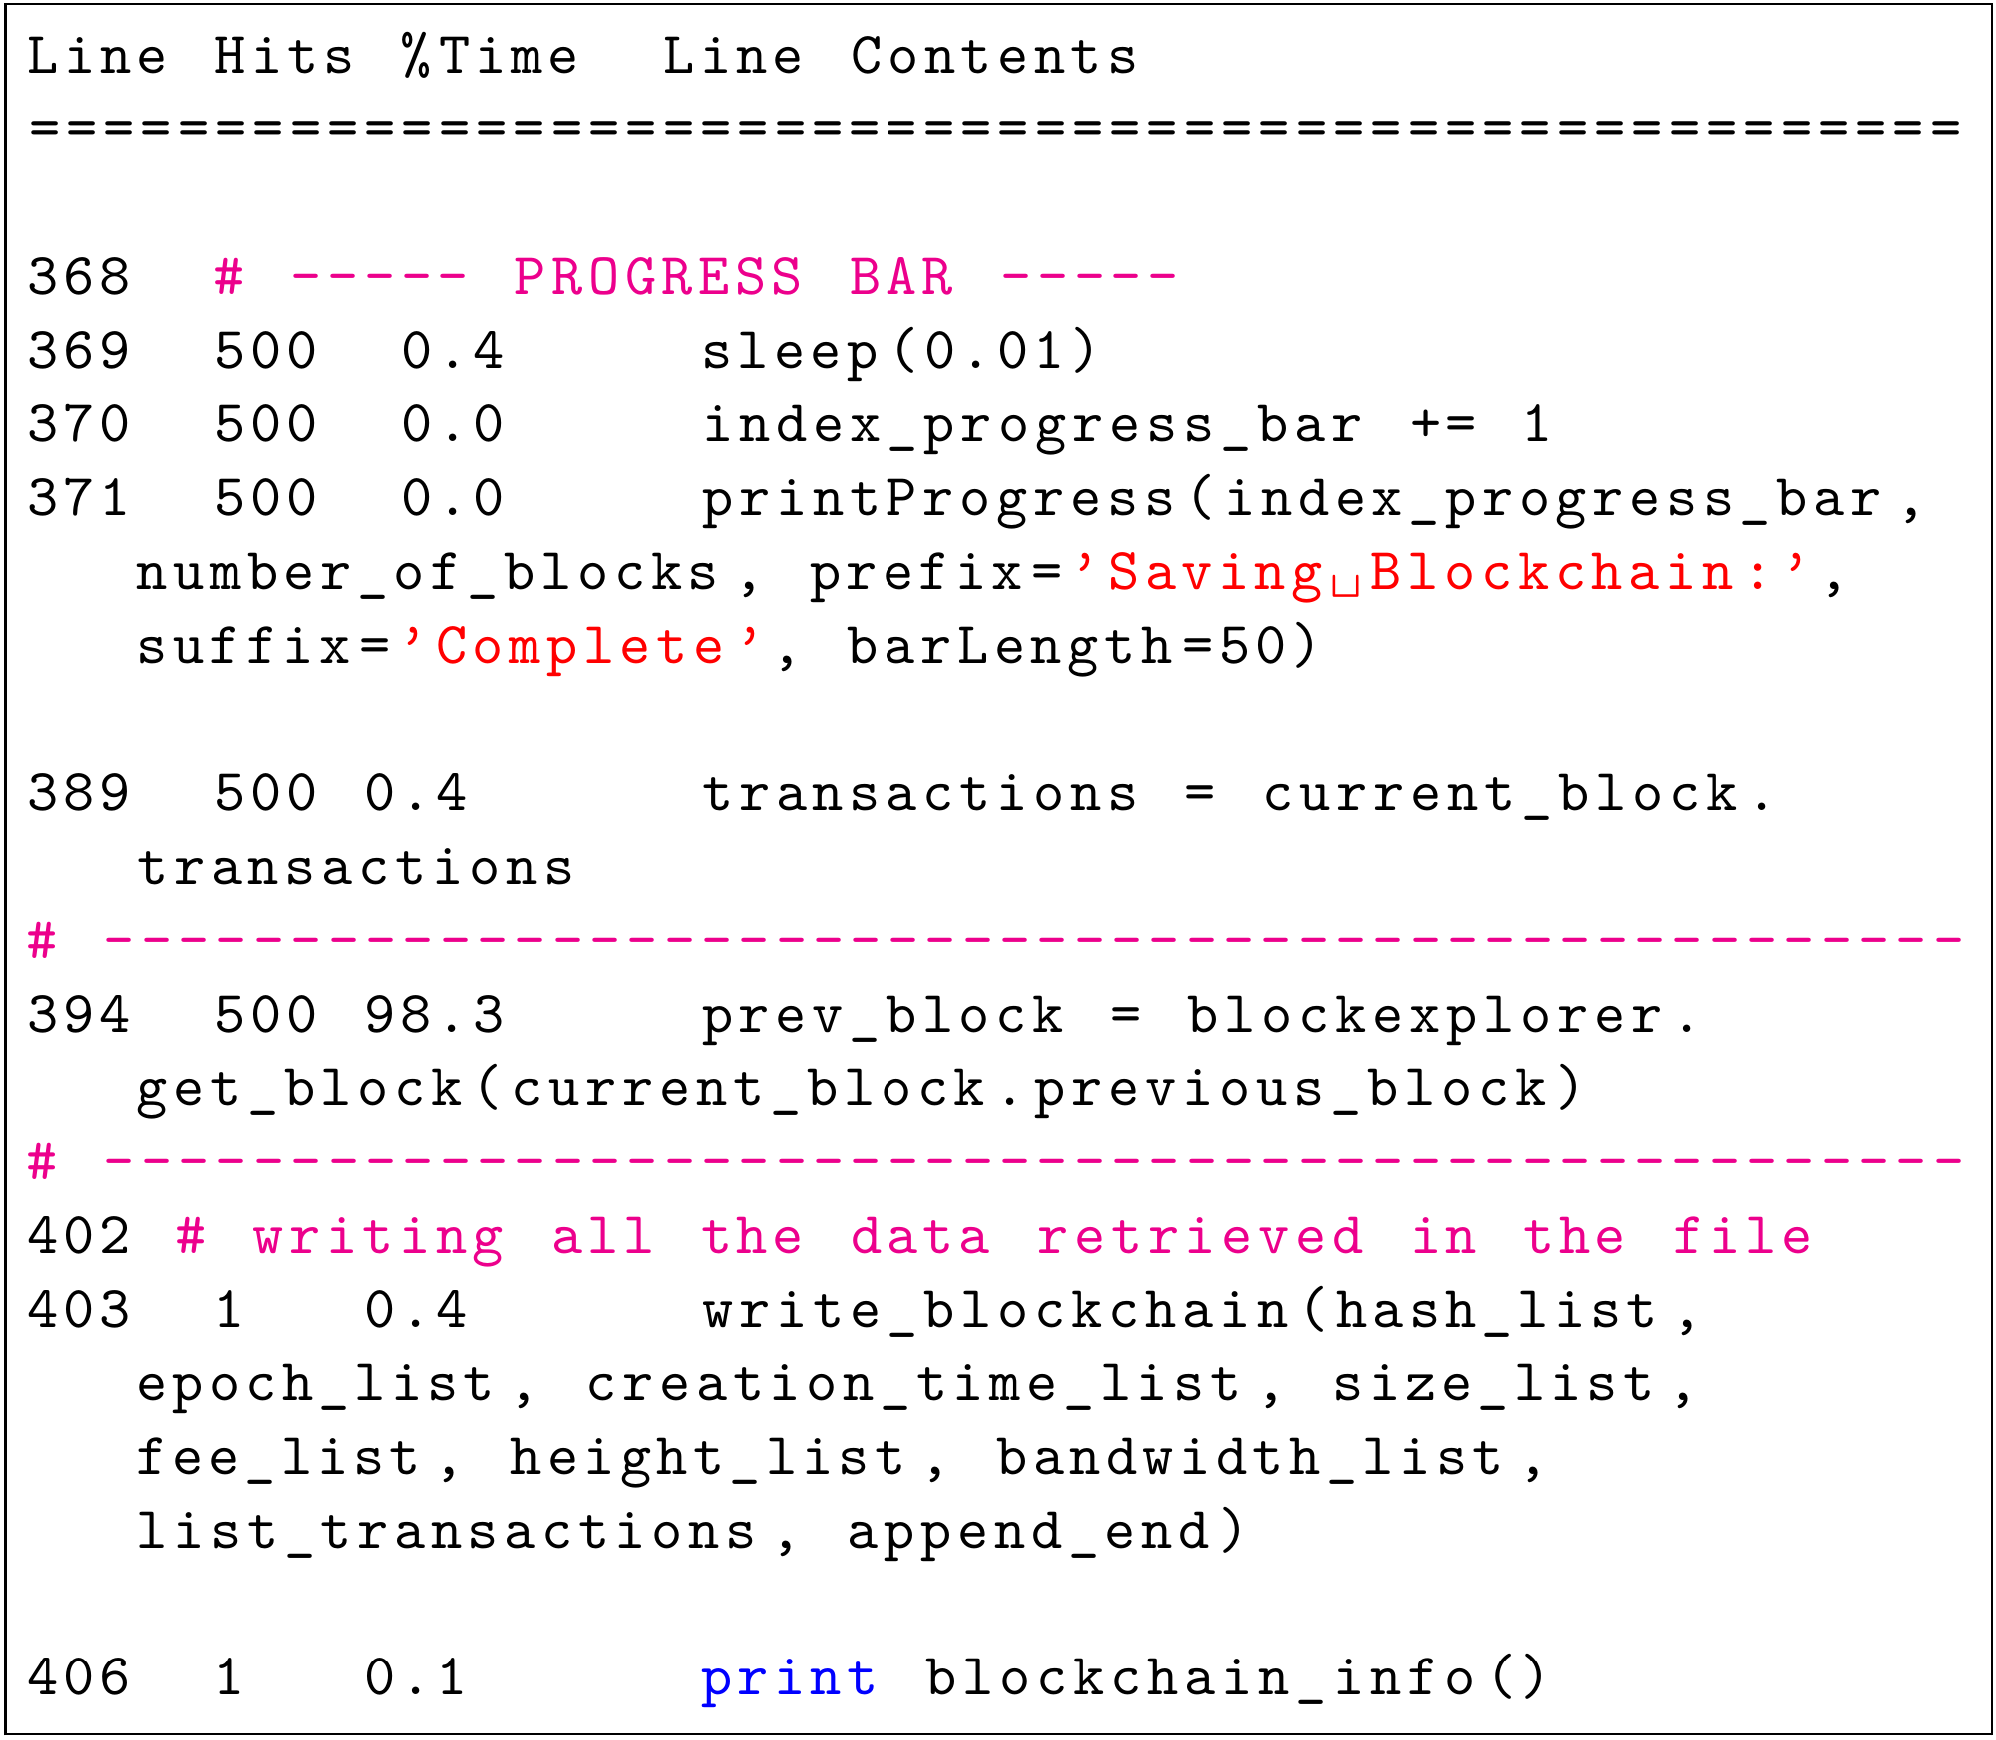
\includegraphics[width=1\textwidth]{img/profile}
%	\caption{Profiling results while executing the system retrieving $500$ blocks}
%	\label{fig:profile}
%\end{figure}
%
%In future implementation more data from each block could be considered, such
%as the correctness of every block created. Correctness for each block is a value obtained
%putting all the most important informations of a block in a multidimensional vector, in the
%following way:
%\begin{equation}
%\label{eq:correctness_vector}
%	C=\begin{bmatrix}
%		B_{sz} \\
%		B_g\\
%		B_s\\
%		B_t
%	\end{bmatrix}
%\end{equation}
%considering for each block the size ($B_{sz}$), the fee ($B_g$), the epoch,
%transformed in creation time ($B_s$) and the
%number of transactions in this block ($B_t$).
%The correctness of a block then is dependent from the range of these values
%and this range can change according to the level of correctness desired.
%For example we could have:
%\begin{equation}
%C_B = \begin{cases}
%300 < B_{sz} \leqslant 1000, & \mbox{bytes} \\
%0.5 < B_g < 1.5, & \mbox{BTC} \\
%6 < B_s < 12, & \mbox{minutes} \\
%500 < B_t < 1500, & \mbox{transactions}
%\end{cases}
%\end{equation}
%Which means that a block is correct if the correctness for this block, $C_B$, respects
%these values. In that way is possible to calculate how many blocks among the
%retrieved ones can be considered correct. It will be also possible to add the percentage
%of each correct/incorrect field, to find any possible relation between those and to get
%information about whether a block is incorrect, why that happened.
%It is already implemented, but not tested yet, the relation between the average
%transaction time and the fee paid to mine a block.
%Furthermore, following the design pattern principles, refactoring on the code must be done since
%the method \emph{write\_blockchain()} contains some \emph{duplicate code} about writing on
%the file. The treatment to use might be \emph{extract method} on the \emph{file.write}.

\section{Comments}
\label{sec:comments}
%A relevant aspect to note is that there are some blocks
%that take approximately $80$\,minutes to be created, when the
%average time is supposed to be $\sim8$\,min. This affects also the
%transaction visibility but it is also a side effect of the difficulty
%and proof of work. Furthermore, the growth of the blockchain
%is not $\sim1$\,MB per hour as claimed from Bitcoin in $2008$
%but, at the moment, $\sim5$\,MB each hour, growing of $\sim2$\,GB in less than $12$\,days.
%In conclusion, we demonstrate our thesis and found a relation between the fee paid to a miner
%and the block creation time. We generate a function which describes this relation and it can
%be used in future implementations, allowing miners to be fairly rewarded.
%A block can arbitrary decides whether ignore a transaction
%that is not willing to pay enough fee ($T_g$).
%Plus, we defined a model for growth prediction and we tested its accuracy. Finally, a portion of
%the blockchain is saved locally and more analysis on it are possible in the future.

show bibliography \cite{Nakamoto_bitcoin}, \cite{ethereum}, \cite{Back02hashcash},
\cite{Dwork:1992}, \cite{Luu:2016}, \cite{Delmolino2016},
\cite{ethereum_white_paper}, \cite{ethereum_solidity}, \cite{Luu:2015:DIC},
\cite{sha}, \cite{Hopcroft:2006:IAT}, \cite{Johansen2015Fireflies}, \cite{bitcoinmining},
\cite{Garcia:2011:EMB}, \cite{vandiver2007hrdb},
\cite{Luiz:2014:MBF}, \cite{bitcoin_api}, \cite{ethereum_api}, \cite{merkle_tree}, \cite{ethereum_wiki_patricia_tree},
\cite{swan2015blockchain}, \cite{Baran1964:ODC}, \cite{Stallings:2002:CNS}, \cite{bitcoin_blockchain}, \cite{ethereum_bc_analysis},
\cite{ethereum_blockchain}, \cite{bitcoinmining_process},
\cite{tradeblock}, \cite{ethereum_website}, \cite{Larman:2004:AUP},
\cite{Aho:1992:FCS}, \cite{matplotlib}, \cite{croman2016}, \cite{DBLP:journals/corr/EyalGSR15},
\cite{Hildebrand:1987:INA}, \cite{mining_hw}, \cite{hashing_rate}, \cite{bitnodes}, \cite{Rizun:2015:blocksizelimit}
\cite{linearize}, \cite{Tedeschi:2016:PBB}, \cite{Donnelly2015BNSB}, \cite{RePEc:gat:wpaper:1407},
\cite{visa}, \cite{DBLP:journals/corr/BartolettiBLP17}, \cite{Moser2015}, \cite{pandas}, \cite{michael_waskom_seaborn}.


\bibliographystyle{plain}
\bibliography{thesis}

\begin{appendices}
	\chapter{Terminology}
	\label{app:terminology}
	\begin{description}
		\item[RLP:] Stands for recursive length prefix. It is a serialization method
		for encoding arbitrary structured binary data (byte arrays).
		\label{item:rlp}
		\item[KEC-256:] Another serialization method generating a 256-bit hash.
		\item[full node:] A full node in a decentralized digital currency peer-2-peer network, is a node that stores
		and processes the entirety of every block, storing locally the entire size of the blockchain.
		\item[light node:] A light node in a decentralized digital currency peer-2-peer network, is a node that only
		stores the part of the blockchain it needs.
		\item[satoshi:] Unit of the Bitcoin currency. 100,000,000 satoshi are 1 BTC (Bitcoin).
	\end{description}

\chapter{List of Symbols}

\begin{description}[leftmargin=!, labelwidth=\widthof{\bfseries $M_{demand}(b)$ }]
	\setlength\itemsep{1em}
	\item [$t_B$] transaction approved in a block $B$.
	\item [$t_{in}$] transaction input in bitcoin (\bitcoin). All the money sent.
	\item [$t_{ou}$] transaction output (\bitcoin). All the money received.
	\item [$t_{f}$] transaction fee (\bitcoin). $t_{in} - t_{ou}$.
	\item [$t_q$] transaction size, in bytes.
	\item [$t_l$] commit latency of a single transaction. $B_{epoch} - t_{epoch}$.
	\item [$\mathcal{T}$] expected block interval time~($\sim$\,$10$\,min)
	\item [$\mathbb{P}_{orphan}$] probability that given a block is orphaned.
	\item [$\tau$] block solution propagation time, we consider a $\tau = 10$\,
	seconds according to Decker\,\cite{Decker2013IPBN}.
	\item [$\eta$] cost per hash.
	\item [$\langle \Pi \rangle$] expectation value of a miner’s profit per block.
	\item [$\langle V\rangle$] expectation value of a miner’s revenue per block.
	\item [$\langle C\rangle$] expectation value of a miner's hashing cost per block.
	\item [$R$] block reward, currently at 12.5 \bitcoin.
	\item [$h$] miner's individual hash rate.
	\item [$H$] total hash rate of Bitcoin network.
	\item [$Q$] block size or block space in bytes.
	\item [$Q^*$] the block size that maximizes the miner’s expected profit.
	\item [$\rho$] fee density, or the price per byte for block space.
	\item [$M$] money, bitcoin (\bitcoin).
	\item [$M_{demand}(b)$] partial sum of the $b$ transaction fees
	in mempool in order of descending fee density.
	\item [$M_{supply}(Q)$] miner’s cost due to orphaning to produce a certain block size $Q$.
	\item [$\mathcal{N}$] the set of transactions in a miner’s mempool.
	\item [$n$] number of transactions in a miner’s mempool.
	\item [$B$] single block.
	\item [$B_t$] transaction root that links to every transaction in a block $B$.
	\item [$B_{epoch}$] timestamp of a block $B$.
	Epoch of when the block was included in the blockchain
	\item [$t_{epoch}$] timestamp of a transaction $t$.
	Epoch of when $t$ was first seen in the network
\end{description}

	\chapter{Listing}
	\label{app:listing}
%	\begin{lstlisting}[numbers=left,frame=single,caption={Smart contract transaction code in Ethereum.}]
%function transfer(address _to, uint256 _value) {
%	/* Add and subtract new balances */
%	balanceOf[msg.sender] -= _value;
%	balanceOf[_to] += _value;
%	}
%	\end{lstlisting}
%	
%	\lstset{language=Python,
%	basicstyle=\ttfamily,
%	keywordstyle=\color{blue}\ttfamily,
%	stringstyle=\color{red}\ttfamily,
%	commentstyle=\color{green}\ttfamily,
%	breaklines=true,
%	morecomment=[l][\color{magenta}]{\#},
%	label = {lst:smartcontract}
%}
%\begin{lstlisting}[float, numbers=left,frame=single,caption={Example of a smart contract that rewards users who solve a computational puzzle~\cite{smartcontracts}.}]
%contract Puzzle {
%  address public owner ;
%  bool public locked ;
%  uint public reward ;
%  bytes32 public diff ;
%  bytes public solution ;
%
%  function Puzzle () // constructor {
%    owner = msg. sender ;
%    reward = msg . value ;
%    locked = false ;
%    diff = bytes32 (11111); // pre - defined difficulty
%    }
%
%  function (){ // main code , runs at every invocation
%    if ( msg. sender == owner ){ // update reward
%    if ( locked )
%    throw ;
%    owner . send ( reward );
%    reward = msg . value ;
%    }
%    else
%      if ( msg . data . length > 0){ // submit a solution
%      if ( locked ) throw ;
%      if ( sha256 (msg. data ) < diff ){
%          msg. sender . send ( reward ); // send reward
%          solution = msg. data ;
%          locked
%          }}}}
%\end{lstlisting}
%
%	\lstset{language=Python,
%	basicstyle=\ttfamily,
%	keywordstyle=\color{blue}\ttfamily,
%	stringstyle=\color{red}\ttfamily,
%	commentstyle=\color{green}\ttfamily,
%	breaklines=true,
%	morecomment=[l][\color{magenta}]{\#},
%	label = {lst:usage}
%}
%\begin{lstlisting}[float, numbers=left, frame=single, caption={Application usage.}]
%Usage: observ.py -t number
%  -h | --help    : usage
%  -i             : gives info of the blockchain in the file .txt
%  -t number      : add on top a number of blocks. The blocks retreived will be the most recent ones. If the blockchain growth more than the block requested do -u (update)
%  -e number      : append blocks at the end of the .txt file. Fetch older blocks starting from the last retrieved
%  -P             : plot all
%  -p start [end] : plot data in .txt file in a certain period of time, from start to end. If only start then consider from start to the end of the .txt file
%  -R             : plot the regression and the models that predict the blockchain
%  -r start [end] : plot the regression and the models in a certain period of time, from start to end. If only start then consider from start to the end of the .txt file
%  -u             : update the local blockchain to the last block created
%
%\end{lstlisting}
%
%
%	\lstset{language=Python,
%	basicstyle=\ttfamily,
%	keywordstyle=\color{blue}\ttfamily,
%	stringstyle=\color{red}\ttfamily,
%	commentstyle=\color{green}\ttfamily,
%	breaklines=true,
%	morecomment=[l][\color{magenta}]{\#},
%	label = {lst:block}
%}
%
%\begin{lstlisting}[float, numbers=left,frame=single,caption={Block object represented in Python according to api-v1-client-python to retrieve data on the blockchain. The function get\_block() will return an object of this type\,\cite{bitcoin_api}.},language=Python]
%class Block:
%  def __init__(self, b):
%    self.hash = b['hash']
%    self.version = b['ver']
%    self.previous_block = b['prev_block']
%    self.merkle_root = b['mrkl_root']
%    self.time = b['time']
%    self.bits = b['bits']
%    self.fee = b['fee']
%    self.nonce = b['nonce']
%    self.n_tx = b['n_tx']
%    self.size = b['size']
%    self.block_index = b['block_index']
%    self.main_chain = b['main_chain']
%    self.height = b['height']
%    self.received_time = b.get('received_time', b['time'])
%    self.relayed_by = b.get('relayed_by')
%    self.transactions = [Transaction(t) for t in b['tx']]
%    for tx in self.transactions:
%        tx.block_height = self.height
%\end{lstlisting}
%
%	\lstset{language=Python,
%	basicstyle=\ttfamily,
%	keywordstyle=\color{blue}\ttfamily,
%	stringstyle=\color{red}\ttfamily,
%	commentstyle=\color{green}\ttfamily,
%	breaklines=true,
%	morecomment=[l][\color{magenta}]{\#},
%	label = {lst:transaction}
%}
%
%\begin{lstlisting}[float, numbers=left,frame=single,caption={Transaction object represented in Python according to api-v1-client-python to retrieve data on the blockchain. The function get\_transaction() will return an object of this type\,\cite{bitcoin_api}.},language=Python]
%class Transaction:
%  def __init__(self, t):
%    self.double_spend = t.get('double_spend', False)
%    self.block_height = t.get('block_height')
%    self.time = t['time']
%    self.relayed_by = t['relayed_by']
%    self.hash = t['hash']
%    self.tx_index = t['tx_index']
%    self.version = t['ver']
%    self.size = t['size']
%    self.inputs = [Input(i) for i in t['inputs']]
%    self.outputs = [Output(o) for o in t['out']]
%
%    if self.block_height is None:
%       self.block_height = -1
%\end{lstlisting}
%
%	\lstset{language=Python,
%	basicstyle=\ttfamily,
%	keywordstyle=\color{blue}\ttfamily,
%	stringstyle=\color{red}\ttfamily,
%	commentstyle=\color{green}\ttfamily,
%	breaklines=true,
%	morecomment=[l][\color{magenta}]{\#},
%	label = {lst:block-json}
%}
%
%\begin{lstlisting}[float, frame=single, caption={Json object returned from the method \emph{get\_block()} in the Bitcoin \gls{api} class blockexplorer.py\,\cite{bitcoin_api}}, language=Python]
%hash : str
%version : int
%previous_block : str
%merkle_root : str
%time : int
%bits : int
%fee : int
%nonce int
%n_tx : int
%size : int
%block_index : int
%main_chain : bool
%height : int
%received_time : int
%relayed_by : string
%transactions : array of Transaction objects
%\end{lstlisting}
%
%
%	\lstset{language=Python,
%	basicstyle=\ttfamily,
%	keywordstyle=\color{blue}\ttfamily,
%	stringstyle=\color{red}\ttfamily,
%	commentstyle=\color{green}\ttfamily,
%	breaklines=true,
%	morecomment=[l][\color{magenta}]{\#},
%	label = {lst:latest-block}
%}
%\begin{lstlisting}[float, numbers=left,frame=single,caption={Structure of the latest block retrieved. The function get\_latest\_block() will return an object with this structure.}]
%class LatestBlock:
%def __init__(self, b):
%self.hash = b['hash']
%self.time = b['time']
%self.block_index = b['block_index']
%self.height = b['height']
%self.tx_indexes = [i for i in b['txIndexes']]
%\end{lstlisting}
%
%
%\lstset{language=Python,
%	basicstyle=\ttfamily,
%	keywordstyle=\color{blue}\ttfamily,
%	stringstyle=\color{red}\ttfamily,
%	commentstyle=\color{green}\ttfamily,
%	breaklines=true,
%	morecomment=[l][\color{magenta}]{\#},
%	label = {lst:append-block}
%}
%\begin{lstlisting}[float, numbers=left, frame=single, caption={Collecting data starting from the last element in the blockchain.txt file.}]
%earliest_hash = get_earliest_hash()
%get_blockchain(n, earliest_hash)
%
%def get_blockchain(n, hash = None):
%  [...]
%  if (hash):  # start the retrieval from the hash
%    append_end = True  # in that way the write_blockchain method knows that has to append blocks and not write them at the beginning
%    last_block = blockexplorer.get_block(hash)
%  [...]
%
%def get_earliest_hash():
%  hash_list = get_list_from_file("hash") # method to collect data from blockchain.txt file having as attribute "hash"
%  length = len(hash_list)
%  earliest_hash = hash_list[length - 1]
%  return earliest_hash
%\end{lstlisting}
%
%
%	\lstset{language=Python,
%	basicstyle=\ttfamily,
%	keywordstyle=\color{blue}\ttfamily,
%	stringstyle=\color{red}\ttfamily,
%	commentstyle=\color{green}\ttfamily,
%	breaklines=true,
%	morecomment=[l][\color{magenta}]{\#},
%	label = {lst:api-python}
%}
%\begin{lstlisting}[float, numbers=left, frame=single,caption={Calling \url{blockchain.info} through python \gls{api} and retrieving part of the blockchain.}]
%from blockchain import blockexplorer
%# get the last block
%last_block = blockexplorer.get_latest_block()
%hash_last_block = last_block.hash
%
%# current block now is the last block
%current_block = blockexplorer.get_block(hash_last_block)
%\end{lstlisting}
%
%	\lstset{language=Python,
%	basicstyle=\ttfamily,
%	keywordstyle=\color{blue}\ttfamily,
%	stringstyle=\color{red}\ttfamily,
%	commentstyle=\color{green}\ttfamily,
%	breaklines=true,
%	morecomment=[l][\color{magenta}]{\#},
%	label = {lst:read-bandwidth},
%	numbers=left,
%	frame=single
%}
%\begin{lstlisting}[float, caption={How read bandwidth is calculated, using the function $datetime.now()$ before and after the \gls{api} call.}]
%start_time = datetime.datetime.now() # ---------
%current_block = blockexplorer.get_block(current_block.previous_block)
%end_time = datetime.datetime.now() # ---------
%time_to_fetch = end_time - start_time
%time_in_seconds = get_time_in_seconds(time_to_fetch)
%
%#latency
%fetch_time_list.append(time_in_seconds)
%
%# calculate Bandwidth with MB/s
%block_size = float(current_block.size) / 1000000
%bandwidth = block_size / time_in_seconds
%bandwidth_list.append(bandwidth)
%\end{lstlisting}
%
%	\lstset{language=Python,
%	basicstyle=\ttfamily,
%	keywordstyle=\color{blue}\ttfamily,
%	stringstyle=\color{red}\ttfamily,
%	commentstyle=\color{green}\ttfamily,
%	breaklines=true,
%	morecomment=[l][\color{magenta}]{\#},
%	label = {lst:get-transaction-time},
%	numbers=left,
%	frame=single
%}
%\begin{lstlisting}[float, caption={Function that get the average write bandwidth of the block, calculating the time for each transaction to be visible in the public ledger of data.}]
%def get_avg_transaction_time(block):
%  # take transactions the block
%  transactions = block.transactions
%
%  # get block time -- when it is visible in the blockchain, so when it was created
%  block_time = block.time
%
%  # list of the creation time for all the transaction in the block
%  transactions_time_list = []
%
%  # list of the time that each transaction needs before being visible in the blockchain
%  time_to_be_visible = []
%
%  for t in transactions:
%    transactions_time_list.append(float(t.time))
%
%  for t_time in transactions_time_list:
%    time_to_be_visible.append(float(block_time - t_time))
%    
%  average_per_block = sum(time_to_be_visible) / len(time_to_be_visible)
%  return average_per_block
%\end{lstlisting}
%
%	\lstset{language=Python,
%	basicstyle=\ttfamily,
%	keywordstyle=\color{blue}\ttfamily,
%	stringstyle=\color{red}\ttfamily,
%	commentstyle=\color{green}\ttfamily,
%	breaklines=true,
%	morecomment=[l][\color{magenta}]{\#},
%	label = {lst:file-write},
%	numbers=left,
%	frame=single
%}
%\begin{lstlisting}[float, caption={How the file.write is performed in the blockchain analytics system. Differences with add and append.}]
%if(append):
%  for i in range(n):
%    file.write("block_informations")
%
%else: # add on top
%  hash_list_in_file = get_list_from_file("hash")
%  first_hash = hash_list_in_file[0]
%  elements = len(hash_list_in_file)
%  last_hash = hash_list_in_file[elements-1]
%  met_first = False
%  with io.FileIO(file_name, "a+") as file:
%    file.seek(0)  # place at the beginning of the file
%    existing_lines = file.readlines()  # read the already existing lines
%    file.seek(0)
%    file.truncate()  # delete all the file
%    file.seek(0)
%    i = 0
%    while (i < n):
%      if (first_hash == hash[i]):
%        met_first = True
%      while((met_first == False) and (i < n)):
%        # append on top
%        file.write("block_informations")
%        i = i + 1
%        if ((i < n) and (first_hash == hash[i])):
%          met_first = True
%      # when the block retrieved meets the one alread in the blockchain write the old file
%      file.writelines(existing_lines)
%
%\end{lstlisting}
%
%	\lstset{language=Python,
%	basicstyle=\ttfamily,
%	keywordstyle=\color{blue}\ttfamily,
%	stringstyle=\color{red}\ttfamily,
%	commentstyle=\color{green}\ttfamily,
%	breaklines=true,
%	morecomment=[l][\color{magenta}]{\#},
%	label = {lst:python-list},
%	numbers=left,
%	frame=single
%}
%\begin{lstlisting}[float, caption={Changing all the values inside a Python list in one code line.}]
%# size_list from byte to MB
%size_list[:] = [x / 1000000 for x in size_list]
%# time_list from seconds in minutes
%time_list[:] = [x / 60 for x in time_list]
%\end{lstlisting}
%
%
%	\lstset{language=Python,
%	basicstyle=\ttfamily,
%	keywordstyle=\color{blue}\ttfamily,
%	stringstyle=\color{red}\ttfamily,
%	commentstyle=\color{green}\ttfamily,
%	breaklines=true,
%	morecomment=[l][\color{magenta}]{\#},
%	label = {lst:get-data-from-file},
%	numbers=left,
%	frame=single
%}
%\begin{lstlisting}[float, caption={Method that allows, given an attribute present in the blockchain.txt file, to create a list containing informations only about this quality using \emph{regular expressions}.}]
%hash_list = get_list_from_file("hash")
%
%def get_list_from_file(attribute):
%  list_to_return = []
%  if (os.path.isfile("blockchain.txt")):
%    # open the file and read in it -- blockchain_file
%    with open("blockchain.txt", "r") as blockchain_file:
%      for line in blockchain_file:
%      # regular expression that puts in a list the line just read: eg. ['hash', '<block_hash>']
%        list = re.findall(r"[\w']+", line)
%        # list[0] --> contains the attribute
%        # list[1] --> contains the value
%        if ((list) and (list[0] == attribute)):
%          list_to_return.append(list[1])
%  return list_to_return
%\end{lstlisting}
%
%	\lstset{language=Python,
%	basicstyle=\ttfamily,
%	keywordstyle=\color{blue}\ttfamily,
%	stringstyle=\color{red}\ttfamily,
%	commentstyle=\color{green}\ttfamily,
%	breaklines=true,
%	morecomment=[l][\color{magenta}]{\#},
%	label = {lst:growing-lists},
%	numbers=left,
%	frame=single
%}
%\begin{lstlisting}[float, caption={Generation of the growing size and time lists. Calculated following the Equations~\ref{eq:growing_size},~\ref{eq:growing_time}.}]
%def create_growing_time_list(time_list):
%  reversed_time_list = time_list[::-1]
%  time_to_append = 0
%  previous_time = 0
%  growing_time_list = []
%  growing_time_list.append(previous_time)
%  for time_el in reversed_time_list:
%    time_to_append = (float(time_el) / (60 * 60)) + previous_time  # time in hours
%    growing_time_list.append(time_to_append)
%    previous_time = time_to_append
%  return growing_time_list
%
%def create_growing_size_list(size_list):
%  reversed_size_list = size_list[::-1]
%  growing_size_list = []
%  value_to_append = 0
%  size_back = 0
%  growing_size_list.append(value_to_append)
%  for size_el in reversed_size_list:
%    value_to_append = size_el + size_back
%    growing_size_list.append(value_to_append)
%    size_back = value_to_append
%  return growing_size_list
%\end{lstlisting}
%
%	\lstset{language=Python,
%	basicstyle=\ttfamily,
%	keywordstyle=\color{blue}\ttfamily,
%	stringstyle=\color{red}\ttfamily,
%	commentstyle=\color{green}\ttfamily,
%	breaklines=true,
%	morecomment=[l][\color{magenta}]{\#},
%	label = {lst:polynomial-interpolation},
%	numbers=left,
%	frame=single
%}
%\begin{lstlisting}[float, caption={Example of a polynomial interpolation of two lists using NumPy libraries.}]
%import numpy as np
%
%model = np.polyfit(list1, list2, deg) # polynomial interpolation between list1 and list2 with the degree of the return polynomial
%# deg = 1 --> linear interpolation
%# deg = 2 --> quadratic
%# deg = 3 --> cubic
%# ...
%predicted = np.polyval(model, list1)
%plt.plot(list1, predicted, 'b-', label="pol_interp")
%\end{lstlisting}
%
%	\lstset{language=Python,
%	basicstyle=\ttfamily,
%	keywordstyle=\color{blue}\ttfamily,
%	stringstyle=\color{red}\ttfamily,
%	commentstyle=\color{green}\ttfamily,
%	breaklines=true,
%	morecomment=[l][\color{magenta}]{\#},
%	label = {lst:check},
%	numbers=left,
%	frame=single
%}
%\begin{lstlisting}[float, caption={Check the status of the local blockhain, True if valid, False if not.}]
%def check_blockchain():
%  check = True
%  list = get_list_from_file("height")
%  number = int(list[0])
%  length_list = len(list)
%  for i in range(length_list):
%    if (number != int(list[i])):
%      check = False
%    number = number - 1
%  return check
%\end{lstlisting}

\end{appendices}

%\begin{itemize}
%\item The first item is a glorious item! It may span several lines and even several paragraphs. Hopefully this spans some lines
%now. Sed feugiat. Cum sociis natoque penatibus et magnis dis parturient montes, nascetur ridiculus mus. Et requiem morbi et nunc. Aliquam dolor odio.
%
%This is the second paragraph of that first item. Gorgeous, gorgeous, gorgeous! Nulla non mauris vitae wisi pisuere convallis. Sed eu nulla nec eros scelerisque pharetra. Nullam varius.
%\item The second item is a peculiar and rather scrumptious item, I would say. Quite, quite interesting.
%\end{itemize}

%\lipsum[7]

%\begin{enumerate}
%\item The first item is a glorious item! It may span several lines and even several paragraphs. Hopefully this spans some lines
%now. Sed feugiat. Cum sociis natoque penatibus et magnis dis parturient montes, nascetur ridiculus mus. Et requiem morbi et nunc. Aliquam dolor odio.
%
%This is the second paragraph of that first item. Gorgeous, gorgeous, gorgeous! Nulla non mauris vitae wisi pisuere convallis. Sed eu nulla nec eros scelerisque pharetra. Nullam varius.
%\item The second item is a peculiar and rather scrumptious item, I would say. Quite, quite interesting.
%\end{enumerate}

%\newpage


%\begin{description}
%\item[Entry A] with definition A.
%\item[Entry B] with definitioin B.
%\item[Entry C] with definition C.
%\end{description}


%\paragraph{A paragraph}
%\lipsum[12]

%\definition{Another definition}


%\begin{table}
%\centering
%\begin{tabular}{|l|l|}
%\hline
%Content left & Content right\\
%\hline
%\end{tabular}
%\caption{Another table}
%\end{table}


%\begin{lstlisting}[frame=single,caption={Small C program},language=C]
%#include "stdio.h"
%#define e 3
%#define g (e/e)
%#define h ((g+e)/2)
%#define f (e-g-h)
%#define j (e*e-g)
%#define k (j-h)
%#define l(x) tab2[x]/h
%#define m(n,a) ((n&(a))==(a))
%
%long tab1[]={ 989L,5L,26L,0L,88319L,123L,0L,9367L };
%int tab2[]={ 4,6,10,14,22,26,34,38,46,58,62,74,82,86 };
%
%main(m1,s) char *s; {
%  int a,b,c,d,o[k],n=(int)s;
%  if(m1==1){ char b[2*j+f-g]; main(l(h+e)+h+e,b);
%    printf(b); }
%  else switch(m1-=h){
%    case f:
%      a=(b=(c=(d=g)<<g)<<g)<<g;
%      return(m(n,a|c)|m(n,b)|m(n,a|d)|m(n,c|d));
%    case h:
%      for(a=f;a<j;++a)
%        if(tab1[a]&&!(tab1[a]%((long)l(n))))
%          return(a);
%    case g:
%      if(n<h)return(g);
%      if(n<j){n-=g;c='D';o[f]=h;o[g]=f;}
%      else{c='\r'-'\b';n-=j-g;o[f]=o[g]=g;}
%      if((b=n)>=e)
%        for(b=g<<g;b<n;++b)o[b]=o[b-h]+o[b-g]+c;
%      return(o[b-g]%n+k-h);
%    default:
%      if(m1-=e) main(m1-g+e+h,s+g); else *(s+g)=f;
%      for(*s=a=f;a<e;) *s=(*s<<e)|main(h+a++,
%      (char *)m1);
%    }
%}
%\end{lstlisting}


\backmatter

\end{document}


%  LocalWords:  cryptocurrency
